% !TEX root = userguide_en.tex
%----------------------------------------------------------
\chapter{File specification}

%----------------------------------------------------------
\section{Input files for Standard mode}
\label{Ch:HowToStandard}

An example of input file for the standard mode is shown below:

\begin{minipage}{10cm}
\begin{screen}
\begin{verbatim}
W = 2
 L = 4
 model = "spin"

 lattice = "triangular lattice"
//mu = 1.0
// t = -1.0
// t' = -0.5
// U = 8.0
//V = 4.0
//V'=2.0
J = -1.0
J'=-0.5
// nelec = 8
\end{verbatim}
\end{screen}
\end{minipage}

{\bf Basic rules for input files}
\begin{itemize}
\item In each line, there is a set of a keyword (before an ``\verb|=|") and a parameter(after an ``\verb|=|"); 
  they are separated by ``\verb|=|".
\item You can describe keywords in a random order.
\item Empty lines and lines beginning in a ``\verb|//|''(comment outs) are skipped.
\item Upper- and lowercase are not distinguished.
  Double quotes and blanks are ignored.
\item There are three kinds of parameters.\\ 
  1.~Parameters that must be specified~(if not, \verb|vmcdry.out| will stop with error messages),\\ 
  2.~Parameters that is not necessary be specified~(if not, default values are used),\\
  3.~Parameters that must not be specified~(if specified, \verb|vmcdry.out| will stop with error messages).\\
  An example of 3 is transfer $t$ for the Heisenberg spin system. 
  If you choose ``model=spin", you should not specify ``$t$".
\end{itemize}

We explain each keywords as follows:

\subsection{Parameters about the kind of a calculation}

\begin{itemize}

\item \verb|model|

  {\bf Type :} String (Choose from \verb|"Fermion Hubbard"|, \verb|"Spin"|, \verb|"Kondo Lattice"|
  %,\verb|"Fermion HubbardGC"|, \verb|"SpinGC"|, \verb|"Kondo LatticeGC"|
  )
%\footnote{GC=Grand Canonical}

{\bf Description :} The target model is specified with this parameter;
\verb|"Fermion Hubbard"| denotes
the canonical ensemble of the Fermion in the Hubbard model
\begin{align}
H = -\mu \sum_{i \sigma} c^\dagger_{i \sigma} c_{i \sigma} 
- \sum_{i \neq j \sigma} t_{i j} c^\dagger_{i \sigma} c_{j \sigma} 
+ \sum_{i} U n_{i \uparrow} n_{i \downarrow}
+ \sum_{i \neq j} V_{i j} n_{i} n_{j},
\label{fml4_1_hubbard}
\end{align}
\verb|"Spin"| denotes canonical ensemble
in the Spin model($\{\sigma_1, \sigma_2\}={x, y, z}$)
\begin{align}
H &= -h \sum_{i} S_{i z} - \Gamma \sum_{i} S_{i x} + D \sum_{i} S_{i z} S_{i z}
\nonumber \\
&+ \sum_{i j, \sigma_1}J_{i j \sigma_1} S_{i \sigma_1} S_{j \sigma_1}+ \sum_{i j, \sigma_1 \neq \sigma_2} J_{i j \sigma_1 \sigma_2} S_{i \sigma_1} S_{j \sigma_2} ,
\label{fml4_1_spin}
\end{align}
\verb|"Kondo Lattice"| denotes canonical ensemble in the Kondo lattice model
\begin{align}
H = - \mu \sum_{i \sigma} c^\dagger_{i \sigma} c_{i \sigma} 
- t \sum_{\langle i j \rangle \sigma} c^\dagger_{i \sigma} c_{j \sigma} 
+ \frac{J}{2} \sum_{i} \left\{
S_{i}^{+} c_{i \downarrow}^\dagger c_{i \uparrow}
+ S_{i}^{-} c_{i \uparrow}^\dagger c_{i \downarrow}
+ S_{i z} (n_{i \uparrow} - n_{i \downarrow})
\right\}.
\label{fml4_1_kondo}
\end{align}
%\verb|"Fermion HubbardGC"|, \verb|"SpinGC"|, and \verb|"Kondo LatticeGC"|
%indicate 
%grand canonical ensemble of the Fermion in the Hubbard model [Eqn. (\ref{fml4_1_hubbard})],
%grand canonical ensemble in the Spin model [Eqn. (\ref{fml4_1_spin})],
%and
%grand canonical ensemble in Kondo lattice model [Eqn. (\ref{fml4_1_kondo})],
%respectively.

\item \verb|lattice|

{\bf Type :} String (Choose from \verb|"Chain Lattice"|, \verb|"Square Lattice"|, 
\verb|"Triangular Lattice"|, \verb|"Honeycomb Lattice"|, \verb|"Kagome"|, \verb|"Ladder"|)

{\bf Description :} The lattice shape is specified with this parameter;
above words denote
the one dimensional chain lattice (Fig. \ref{fig_chap04_1_lattice}(a)), 
the two dimensional square lattice (Fig. \ref{fig_chap04_1_lattice}(b)),
the two dimensional triangular lattice (Fig. \ref{fig_chap04_1_lattice}(c)),
the two dimensional anisotropic honeycomb lattice (Fig. \ref{fig_chap04_1_honeycomb}),
the Kagome Lattice(Fig. \ref{fig_kagome}),
and
the ladder lattice (Fig. \ref{fig_ladder}),
respectively.

\begin{figure}[!tbhp]
  \begin{center}
    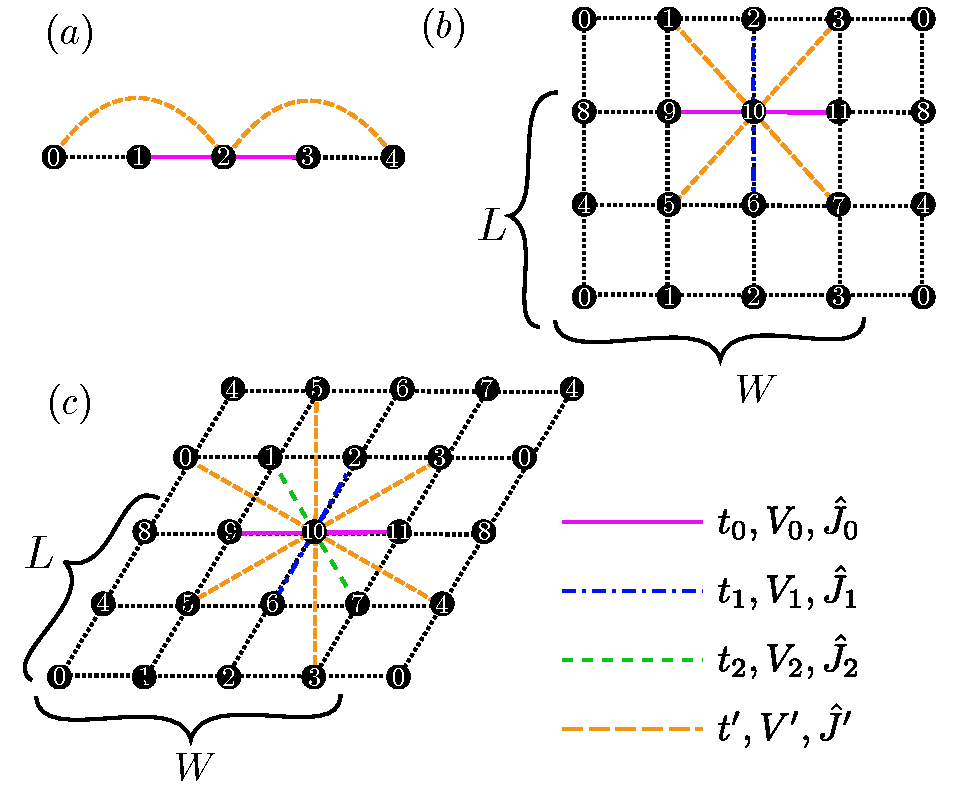
\includegraphics[width=15cm]{../figs/chap04_1_lattice.pdf}
    \caption{Schematic illustration of
      (a) one dimensional chain lattice, 
      (b) two dimensional square lattice, and 
      (c) two dimensional triangular lattice.
      They have $t$, $V$, and $J$ as a nearest neighbor hopping, an offsite Coulomb integral, 
      and a spin-coupling constant, respectively (magenta solid lines);
      They also have $t'$, $V'$, and $J'$ as a next nearest neighbor hopping, offsite Coulomb integral, 
      and spin-coupling constant, respectively (green dashed line).
    }
    \label{fig_chap04_1_lattice}
  \end{center}
\end{figure}

\begin{figure}[!tbhp]
  \begin{center}
    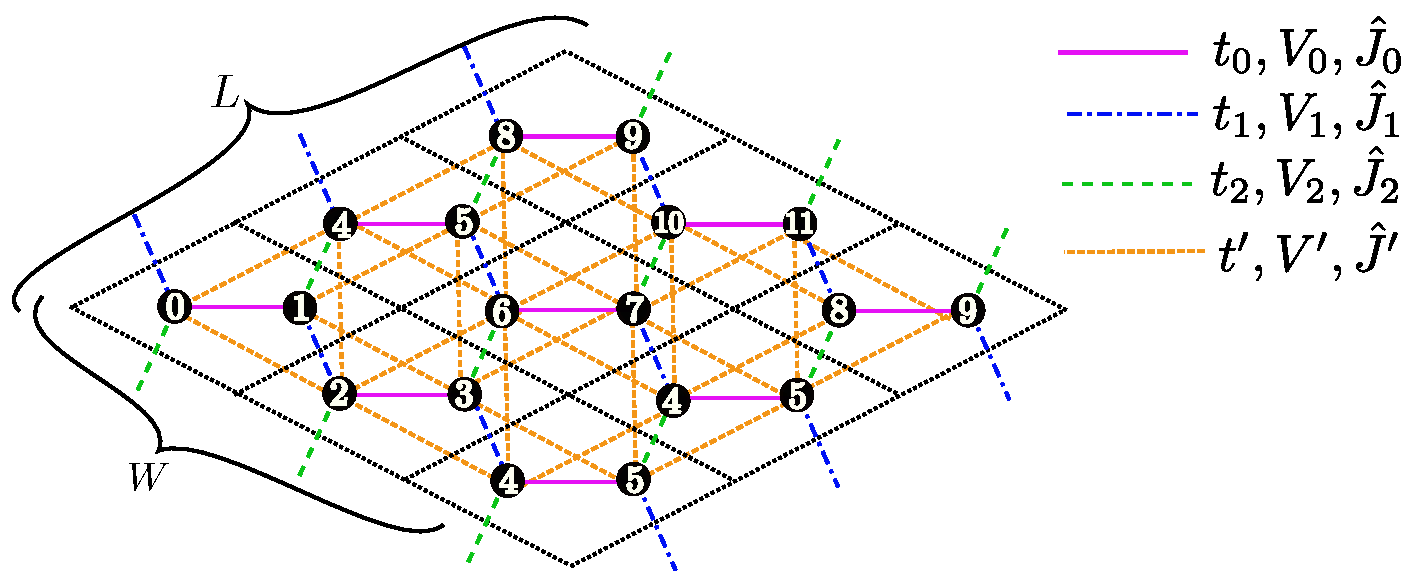
\includegraphics[width=15cm]{../figs/chap04_1_honeycomb.pdf}
    \caption{Schematic illustration of the anisotropic honeycomb lattice.
      The nearest neighbor 
      hopping integral, spin coupling, offsite Coulomb integral
      depend on the bond direction.
      Those between second nearest neighbor sites are not supported.
    }
    \label{fig_chap04_1_honeycomb}
  \end{center}
\end{figure}

\begin{figure}[!tbhp]
  \begin{center}
    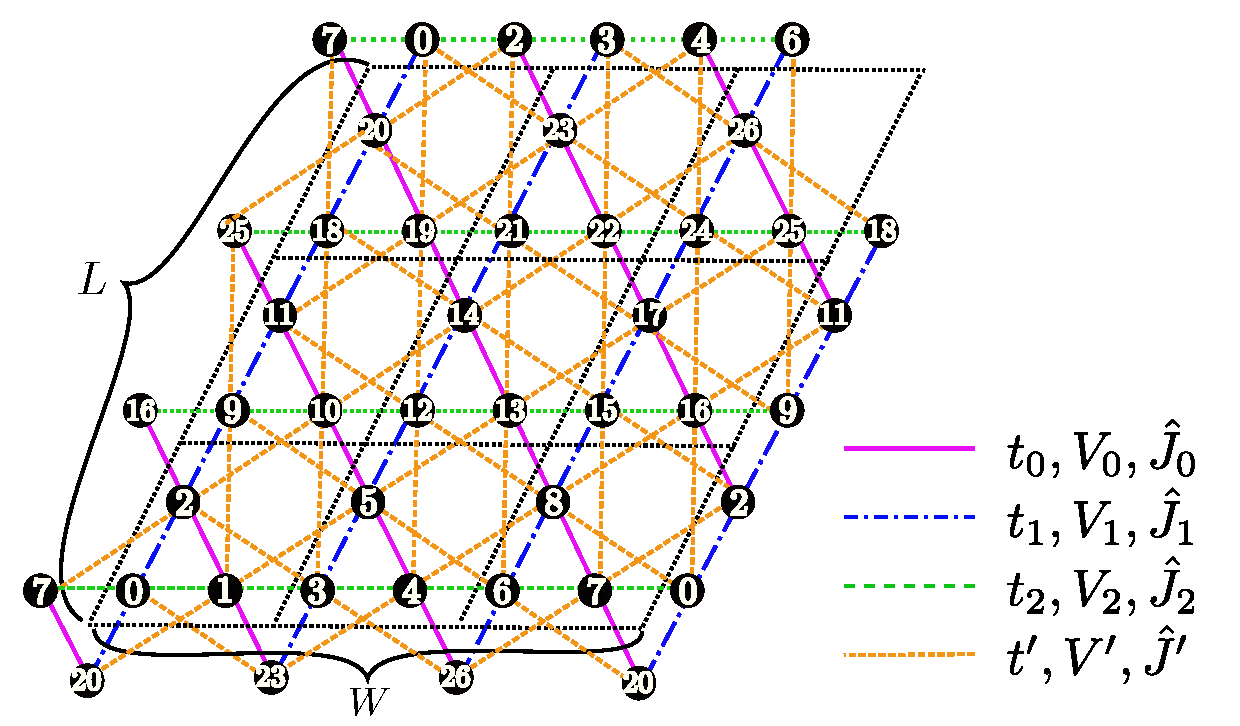
\includegraphics[width=10cm]{../figs/kagome.pdf}
    \caption{Schematic illustration of the Kagome lattice.
    }
    \label{fig_kagome}
  \end{center}
\end{figure}

\begin{figure}[!tbhp]
  \begin{center}
    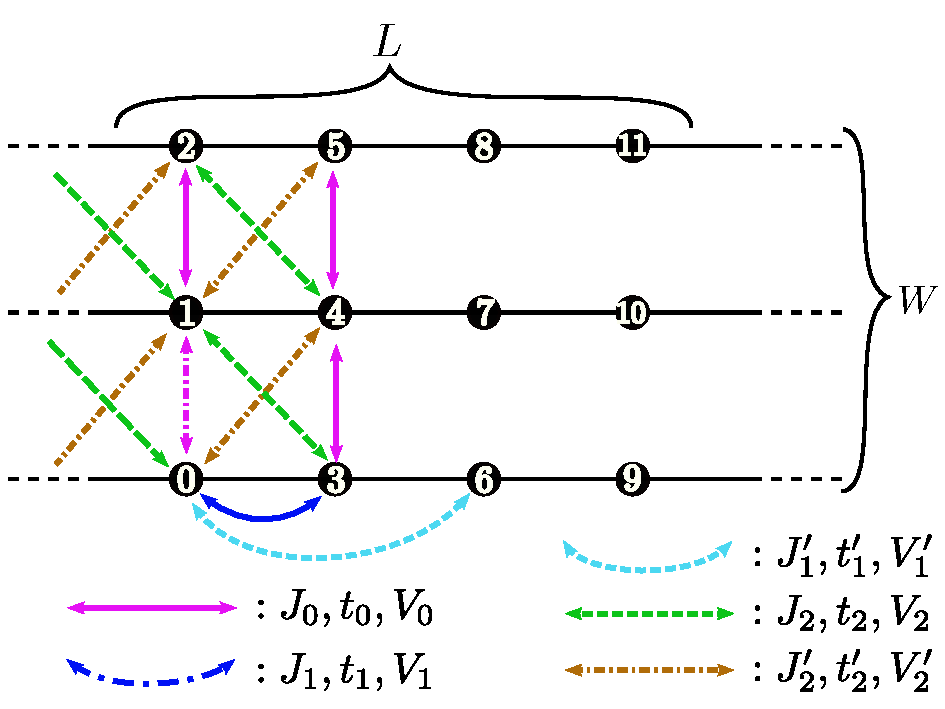
\includegraphics[width=10cm]{../figs/ladder.pdf}
    \caption{Schematic illustration of the ladder lattice.
    }
    \label{fig_ladder}
  \end{center}
\end{figure}

\end{itemize}

\subsection{Parameters for the lattice}

\subsubsection{Chain [Fig. \ref{fig_chap04_1_lattice}(a)]}

\begin{itemize}

\item \verb|L|

{\bf Type :} Integer

{\bf Description :} The length of the chain is specified 
with this parameter.

\end{itemize}

\subsubsection{Ladder (Fig. \ref{fig_ladder})}

\begin{itemize}

\item \verb|L|

{\bf Type :} Integer

{\bf Description :} The length of the ladder is specified 
with this parameter.

\item \verb|W|

{\bf Type :} Integer

{\bf Description :} The number of the ladder is specified 
with this parameter.

\end{itemize}

\begin{figure}[!tbhp]
  \begin{center}
    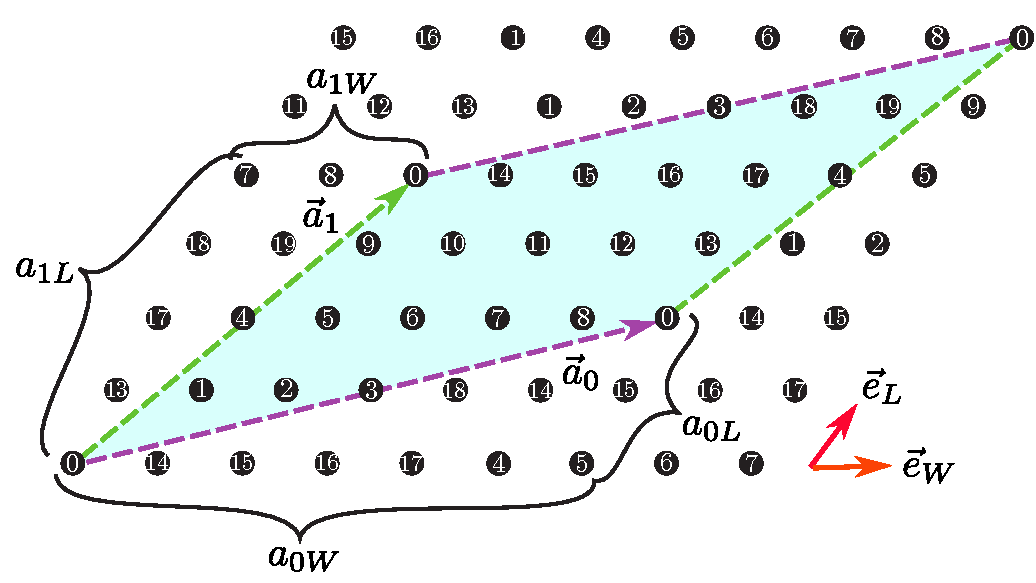
\includegraphics[width=15cm]{../figs/chap04_1_unitlattice.pdf}
    \caption{The shape of the numerical cell 
      when ${\vec a}_0 = (6, 2), {\vec a}_1 = (2, 4)$
      in the triangular lattice.
      The region surrounded by 
      ${\vec a}_0$(Magenta dashed arrow) and ${\vec a}_1$(Green dashed arrow)
      becomes the cell to be calculated (20 sites).
    }
    \label{fig_chap04_1_unitlattice}
  \end{center}
\end{figure}

\subsubsection{Square lattice [Fig. \ref{fig_chap04_1_lattice}(b)], 
Triangular lattice[Fig. \ref{fig_chap04_1_lattice}(c)],
Honeycomb lattice(Fig. \ref{fig_chap04_1_honeycomb}),
Kagome lattice(Fig. \ref{fig_kagome})}

In these lattices,
we can specify the shape of the numerical cell by using the following two methods.

\begin{itemize}

\item \verb|W|, \verb|L|

{\bf Type :} Integer

{\bf Description :} The alignment of original unit cells 
(dashed black lines in Figs. \ref{fig_chap04_1_lattice} - \ref{fig_kagome})
is specified with these parameter.

\item \verb|a0W|, \verb|a0L|, \verb|a1W|, \verb|a1L|

{\bf Type :} Integer

{\bf Description :} 
We can specify two vectors (${\vec a}_0, {\vec a}_1$)
that surrounds the numerical cell (Fig. \ref{fig_chap04_1_unitlattice}).
These vectors should be specified in the Fractional coordinate.

\end{itemize}

If we use both of these method, \verb|vmcdry.out| stops.

We can check the shape of the numerical cell
by using a file \verb|lattice.gp|(only for
square, trianguler, honeycomb, and kagome lattice)
which is written in the Standard mode.
This file can be read by \verb|gnuplot| as follows:
\begin{verbatim}
$ gnuplot lattice.gp
\end{verbatim}

\subsection{Sublattice}

By using the following parameters, we can force the pair-orbital symmetrical
to the translation of the sublattice.

\begin{itemize}

\item \verb|a0Wsub|, \verb|a0Lsub|, \verb|a1Wsub|, \verb|a1Lsub|, \verb|Wsub|, \verb|Lsub|

{\bf Type :} Positive integer. In the default setting, 
\verb|a0Wsub=a0W|, \verb|a0Lsub=a0L|, \verb|a1Wsub=a1W|, \verb|a1Lsub=a1L|, 
\verb|Wsub=W|, and \verb|Lsub=L|. Namely, there is no sublattice.

{\bf Description :} We can specify these parameter as we specify
\verb|a0W|, \verb|a0L|, \verb|a1W|, \verb|a1L|, \verb|W|, \verb|L|.
If the sublattice is incommensurate with the original lattice,
\verb|vmcdry.out| stops.

\end{itemize}

\subsection{Parameters for the Hamiltonian}
A default value is set as $0$ unless a specific value is not defined in a description. 
Table~\ref{table_interactions} shows the parameters for each models. 
In the case of a complex type, a file format is ``{\it a real part, an imaginary part} "
 while in the case of a real type, only ``{\it a real part} ".

\subsubsection{Local terms}

\begin{itemize}

\item \verb|mu|

{\bf Type :} Real

{\bf Description :} (Hubbard and Kondo lattice model) 
The chemical potential $\mu$ (including the site potential)
is specified with this parameter.

\item \verb|U|

{\bf Type :} Real

{\bf Description :} (Hubbard and Kondo lattice model) 
The onsite Coulomb integral $U$ is specified with this parameter.

\item \verb|Jx|, \verb|Jy|, \verb|Jz|, \verb|Jxy|, 
  \verb|Jyx|, \verb|Jxz|, \verb|Jzx|, \verb|Jyz|, \verb|Jzy|

{\bf Type :} Real

{\bf Description :} (Kondo lattice model) 
The spin-coupling constant between the valence and the local electrons
is specified with this parameter.
If the exchange coupling \verb|J| is specified in the input file,
instead of \verb|Jx, Jy, Jz|,
the diagonal exchange couplings, \verb|Jx, Jy, Jz|, are set as \verb|Jx = Jy = Jz = J|.
When both
the set of exchange couplings (\verb|Jx|, \verb|Jy|, \verb|Jz|)
and the exchange coupling \verb|J| are specified in the input file,
\verb|vmcdry.out| will stop.

\item \verb|h|, \verb|Gamma|, \verb|D|

{\bf Type :} Real

{\bf Description :} (Spin model)
The longitudinal magnetic field, transverse magnetic field, 
and the single-site anisotropy parameter are specified with these parameters.
The single-site anisotropy parameter is not available for \verb|model=SpinGCBoost|.

\end{itemize}

The non-local terms described below should be specified
in different ways depending on the lattice structure:
For \verb|lattice=Ladder|, the non-local terms are specified in the different way
from \verb|lattice=Chain Lattice|, \verb|Square Lattice|, \verb|Triangular Lattice|, \verb|Honeycomb Lattice|, \verb|Kagome|. 
Below, the available parameters for each lattice are shown in
Table \ref{table_interactions}.

\begin{table}[tbhp]
  \begin{tabular}{|l||c|c|c|c|c|c|c|c|} \hline
    Interactions & 1D chain & 2D square & 2D triangular & Honeycomb & Kagome & Ladder\\ 
    \hline 
    \hline
     \verb|J|, \verb|t|, \verb|V| (simplified) & $\circ$	 & $\circ$ & $\circ$ & $\circ$ & $\circ$ & -\\ 
     \hline
    \verb|J'|, \verb|t'|, \verb|V'| & $\circ$	 & $\circ$	& $\circ$ 	& $\circ$ 	& $\circ$ & - \\ 
    \hline
    \verb|J0|, \verb|t0|, \verb|V0| & $\circ$  & $\circ$ 	& $\circ$ 	& $\circ$ 	& $\circ$ & $\circ$\\ 
    \hline
    \verb|J1|, \verb|t1|, \verb|V1| & -         	 & $\circ$ 	& $\circ$ 	& $\circ$ 	& $\circ$ & $\circ$\\ 
    \hline
    \verb|J2|, \verb|t2|, \verb|V2|  & -         	 & -    	& $\circ$ 	& $\circ$ 	& $\circ$ & $\circ$\\
    \hline
    \verb|J1'|, \verb|t1'|, \verb|V1'| & -		 &-	 	& -		& -		& -		& $\circ$\\
    \hline
    \verb|J2'| ,\verb|t2'|, \verb|V2'|  & -		 &-	 	& -		& -		& -		& $\circ$\\ 
    \hline
\end{tabular}
   \caption{Interactions for each models defined in an input file. We can define spin couplings as matrix format.}
    \label{table_interactions}
\end{table}

\subsubsection{Non-local terms[ for Ladder (Fig. \ref{fig_ladder})]}

\begin{itemize}
\item \verb|t0|,  \verb|t1|,  \verb|t1'|,  \verb|t2|,  \verb|t2'|

{\bf Type :} Complex

{\bf Description :} (Hubbard and Kondo lattice model)
Hopping integrals in the ladder lattice 
(See Fig. \ref{fig_ladder}) is specified with this parameter.

\item \verb|V0|,  \verb|V1|,  \verb|V1'|,  \verb|V2|,  \verb|V2'|

{\bf Type :} Real

{\bf Description :} (Hubbard and Kondo lattice model)
Offsite Coulomb integrals on the ladder lattice
(Fig. \ref{fig_chap04_1_honeycomb} are specified with these parameters.

\item \verb|J0x|, \verb|J0y|, \verb|J0z|, \verb|J0xy|, 
  \verb|J0yx|, \verb|J0xz|, \verb|J0zx|, \verb|J0yz|, \verb|J0zy|
\item \verb|J1x|, \verb|J1y|, \verb|J1z|, \verb|J1xy|, 
  \verb|J1yx|, \verb|J1xz|, \verb|J1zx|, \verb|J1yz|, \verb|J1zy|
\item \verb|J1'x|, \verb|J1'y|, \verb|J1'z|, \verb|J1'xy|, 
  \verb|J1'yx|, \verb|J1'xz|, \verb|J1'zx|, \verb|J1'yz|, \verb|J1'zy|
\item \verb|J2x|, \verb|J2y|, \verb|J2z|, \verb|J2xy|, 
  \verb|J2yx|, \verb|J2xz|, \verb|J2zx|, \verb|J2yz|, \verb|J2zy|
\item \verb|J2'x|, \verb|J2'y|, \verb|J2'z|, \verb|J2'xy|, 
  \verb|J2'yx|, \verb|J2'xz|, \verb|J2'zx|, \verb|J2'yz|, \verb|J2'zy|

{\bf Type :} Real

{\bf Description :} (Spin model)
Spin-coupling constants in the ladder lattice
(See Fig. \ref{fig_ladder}) are specified with these parameter.
If the simplified parameter \verb|J0| is specified in the input file instead of
the diagonal couplings, \verb|J0x, J0y, J0z|,
these diagonal couplings are set as \verb|J0x = J0y = J0z = J0|.
If both \verb|J0| and the set of the couplings (\verb|J0x, J0y, J0z|)
are specified, \verb|vmcdry.out| will stop.
The above rules are also valid for the simplified parameters, \verb|J1|, \verb|J1'|, \verb|J2|, and \verb|J2'|.

\end{itemize}

\subsubsection{Non-local terms [other than Ladder (Figs. \ref{fig_chap04_1_lattice}, \ref{fig_chap04_1_honeycomb},
\ref{fig_kagome})]}

\begin{itemize}
\item \verb|t0|,  \verb|t1|, \verb|t2|

{\bf Type :} Complex

{\bf Description :} (Hubbard and Kondo lattice model)
Nearest neighbor hoppings for each direction
(See Figs. \ref{fig_chap04_1_lattice}-\ref{fig_kagome}.
These bonds are depicted with different line styles.)
are specified with these parameter.
If there is no bond dependence of the nearest-neighbor hoppings,
the simplified parameter \verb|t| is available to specify \verb|t0|,  \verb|t1|, and \verb|t2| as
\verb|t0 = t1 = t2 = t|.
If both \verb|t| and the set of the hoppings (\verb|t0|,  \verb|t1|, \verb|t2|) are specified,
\verb|vmcdry.out| will stop.

\item \verb|V0|,  \verb|V1|, \verb|V2|

{\bf Type :} Real

{\bf Description :} (Hubbard and Kondo lattice model)
Nearest-neighbor offsite Coulomb integrals $V$
 for each direction
 (See Figs. \ref{fig_chap04_1_lattice}-\ref{fig_kagome}.
 These bonds are depicted with different line styles.)
are specified with these parameters.
If there is no bond dependence of the nearest-neighbor offsite Coulomb integrals,
the simplified parameter \verb|V| is available to specify \verb|V0|,  \verb|V1|, and \verb|V2| as
\verb|V0 = V1 = V2 = V|.
If both \verb|V| and the set of the Coulomb integrals (\verb|V0|,  \verb|V1|, \verb|V2|) are specified,
\verb|vmcdry.out| will stop.

\item \verb|J0x|, \verb|J0y|, \verb|J0z|, \verb|J0xy|, 
  \verb|J0yx|, \verb|J0xz|, \verb|J0zx|, \verb|J0yz|, \verb|J0zy|
\item \verb|J1x|, \verb|J1y|, \verb|J1z|, \verb|J1xy|, 
  \verb|J1yx|, \verb|J1xz|, \verb|J1zx|, \verb|J1yz|, \verb|J1zy|
\item \verb|J2x|, \verb|J2y|, \verb|J2z|, \verb|J2xy|, 
  \verb|J2yx|, \verb|J2xz|, \verb|J2zx|, \verb|J2yz|, \verb|J2zy|

{\bf Type :} Real

{\bf Description :} (Spin model)
Nearest-neighbor exchange couplings for each direction
are specified with thees parameters.
If the simplified parameter \verb|J0| is specified, instead of \verb|J0x, J0y, J0z|,
the exchange couplings, \verb|J0x, J0y, J0z|, are set as \verb|J0x = J0y = J0z = J0|.
If both \verb|J0| and the set of the exchange couplings (\verb|J0x, J0y, J0z|)
are specified, \verb|vmcdry.out| will stop.
The above rules are valid for \verb|J1| and \verb|J2|.

If there is no bond dependence of the nearest-neighbor exchange couplings,
the simplified parameters,
\verb|Jx|, \verb|Jy|, \verb|Jz|, \verb|Jxy|, 
\verb|Jyx|, \verb|Jxz|, \verb|Jzx|, \verb|Jyz|, \verb|Jzy|,
are available to specify the exchange couplings for every bond as
\verb|J0x = J1x = J2x = Jx|.
If any simplified parameter (\verb|Jx|$\sim$\verb|Jzy|)
is specified in addition to its counter parts (\verb|J0x|$\sim$\verb|J2zy|),
\verb|vmcdry.out| will stop.
Below, examples of parameter sets for nearest-neighbor exchange couplings are shown.

\begin{itemize}

\item If there are no bond-dependent, no anisotropic and offdiagonal exchange couplings (such as $J_{x y}$),
please specify \verb|J| in the input file.

\item If there are no bond-dependent and offdiagonal exchange couplings
but are anisotropic couplings,
please specify the non-zero couplings in the diagonal parameters, \verb|Jx, Jy, Jz|.

\item If there are no bond-dependent exchange couplings
but are anisotropic and offdiagonal exchange couplings,
please specify the non-zero couplings in the nine parameters,
\verb|Jx, Jy, Jz, Jxy, Jyz, Jxz, Jyx, Jzy, Jzx|.

\item If there are no anisotropic and offdiagonal exchange couplings,
but are bond-dependent couplings,
please specify the non-zero couplings in the three parameters,
\verb|J0, J1, J2|.

\item If there are no anisotropic exchange couplings, but are bond-dependent and offdiagonal couplings,
please specify the non-zero couplings in the nine parameters,
\verb|J0x, J0y, J0z, J1x, J1y, J1z, J2x, J2y, J2z|.

\item If there are bond-dependent, anisotropic and offdiagonal exchange couplings,
please specify the non-zero couplings in the twenty-seven parameters from
\verb|J0x| to \verb|J2zy|.

\end{itemize}
\item \verb|t'|

{\bf Type :} Complex

{\bf Description :} (Hubbard and Kondo lattice model)
Nearest neighbor hoppings for each direction
(See Figs. \ref{fig_chap04_1_lattice}-\ref{fig_kagome})
are specified with these parameter.

\item \verb|V'|

{\bf Type :} Real

{\bf Description :} (Hubbard and Kondo lattice model)
Nearest neighbor-offsite Coulomb integrals $V$
 for each direction
(See Figs. \ref{fig_chap04_1_lattice}-\ref{fig_kagome})
are specified with these parameters.

\item \verb|J'x|, \verb|J'y|, \verb|J'z|, \verb|J'xy|, 
  \verb|J'yx|, \verb|J'xz|, \verb|J'zx|, \verb|J'yz|, \verb|J'zy|

{\bf Type :} Real

{\bf Description :} (Spin model)
Second nearest-neighbor exchange couplings are specified.
However, for \verb|lattice = Honeycomb Lattice| and  \verb|lattice = Kagome|
with \verb|model=SpinGCBoost|,
the second nearest-neighbor exchange couplings are not available in the $Standard$ mode.
If the simplified parameter \verb|J'| is specified, instead of
\verb|J'x, J'y, J'z|,
the exchange couplings are set as
\verb|J'x = J'y = J'z = J'|.
If both \verb|J'| and the set of the couplings (\verb|J'x, J'y, J'z|),
\verb|vmcdry.out| will stop.

\item \verb|phase0|, \verb|phase1|

  {\bf Type :} Double complex (\verb|1.0| as defaults)
  
  {\bf Description :}
  We can specify the phase for the prefactor for the hopping through the cell boundary
  with these parameter.
  These fuctor for the $\vec{a}_0$ direction and the $\vec{a}_1$ direction can be specified independently.
  For the one-dimensional system, only \verb|phase0| can be used.
  For example, a fopping from $i$-th site to $j$-th site through the cell boundary with the positive direction
  becomes as 
  \begin{align}
    \exp(i \times {\rm phase0}) \times t {\hat c}_{j \sigma}^\dagger {\hat c}_{i \sigma}
    + \exp(-i \times {\rm phase0}) \times t^* {\hat c}_{i \sigma}^\dagger {\hat c}_{j \sigma}
  \end{align}

\end{itemize}

\subsection{Parameters for the numerical condition}

\begin{itemize}

\item  \verb|nelec|

  {\bf Type :} {int-type (must be specified)}

  {\bf Description :} {The number of itenerant electrons.
    It is the sum of the $\uparrow$ and $\downarrow$ electrons.}

\item  \verb|NVMCCalMode|

 {\bf Type :} int-type (default value: 0)

{\bf Description :} [0] Optimization of variational parameters, [1] Calculation of one body and two body Green's functions.

% \item  \verb|NLanczosMode|

% {\bf Type :} int-type (default value: 0)

%{\bf Description :} [0] Not using single Lanczos step, [1] Calculating energy by using Single Lanczos Step, [2] Calculating one body and two body Green's functions by using Single Lanczos Step (Condigion: The options 1 and 2 can be selected when \verb|NVMCCalMode| = 1. When Hamiltonian includes  pair hopping or exchange terms, the options 1 and 2 cannot be used).
 
 \item  \verb|NDataIdxStart|

 {\bf Type :} int-type (default value: 1)

{\bf Description :} An integer for numbering of output files. For \verb|NVMCCalMode|= 0 , \verb|NDataIdxStart| is added at the end of the output files. For \verb|NVMCCalMode| = 1,  the files are outputted with the number from \verb|NDataIdxStart| to  \verb|NDataIdxStart|+\verb|NDataQtySmp|-1.
   
 \item  \verb|NDataQtySmp|

 {\bf Type :} int-type (default value: 1)

{\bf Description :} The set number for outputted files (only used for \verb|NVMCCalMode| = 1). 

 \item  \verb|NSPGaussLeg|

{\bf Type :} {int-type (Positive integer, default value: 1)}

{\bf Description :} The mesh number for the Gauss-legendre quadrature about $\beta$ integration ($S_y$ rotation) for the spin quantum-number projection in actual numerical calculation.

 \item  \verb|NSPStot|

{\bf Type :} int-type ( greater than 0,  default value: 0)

{\bf Description :}   The spin quantum-number. 

\item  \verb|NMPTrans|

  {\bf Type :} int-type (Positive integer.
  As a defalut, The number of translational vectors in the sublattice)

  {\bf Description :} 
  The number of the momentum and lattice translational quantum-number projection.
  In the case of not to apply the projection, this value must be set as 1.

 \item  \verb|NSROptItrStep|

{\bf Type :} int-type (Positive integer, default value: 1000)

{\bf Description :} 
The whole step number to optimize variational parameters by SR method. Only used for \verb|NVMCCalMode|=0.
 
 \item  \verb|NSROptItrSmp|

{\bf Type :} int-type (Positive integer, default value: \verb|NSROptItrStep|/10)

{\bf Description :} In the \verb|NSROptItrStep| step, the average values of the each variational parameters at the \verb|NSROptItrStep| step are adopted as the optimized values. Only used for \verb|NVMCCalMode|=0.

\item   \verb|DSROptRedCut|
   
{\bf Type :} double-type (default value: 0.001)

{\bf Description :} The stabilized factor for the SR method by truncation of redundant directions corresponding to $\varepsilon_{\rm wf}$ in the ref. \cite{Tahara2008}.

 \item  \verb|DSROptStaDel| 
   
 {\bf Type :} double-type (default value: 0.02)

  {\bf Description :} The stabilized factor for the SR method by modifying diagonal elements in the overwrap matrix corresponding to $\varepsilon$ in the ref. \cite{Tahara2008}.
     
\item \verb|DSROptStepDt|

{\bf Type :} double-type (default value: 0.02)

{\bf Description :} The time step using in the SR method. 
 
\item \verb|NVMCWarmUp|

{\bf Type :} int-type (Positive integer, default value: 10)

{\bf Description :} Idling number for the Malkov chain Montecarlo Methods.

\item \verb|NVMCInterval|

{\bf Type :} int-type (Positive integer, default value: 1)

{\bf Description :} The interval step between samples. The local update will be performed \verb|Nsite|× \verb|NVMCInterval| times.

\item \verb|NVMCSample|

{\bf Type :} int-type (Positive integer, default value: 1000)

{\bf Description :} The sample numbers to calculate the expected values.

\item \verb|NExUpdatePath|

{\bf Type :} int-type (Positive integer)

{\bf Description :}  The option for local update about exchange terms. 0: not update, 1: update. The default value is set as 1 when the local spin exists, otherwise 0.

\item \verb|RndSeed|

{\bf Type :} int-type (default value: 123456789)

{\bf Description :} The initial seed of generating random number. For MPI parallelization, the initial seeds are given by \verb|RndSeed|+my rank+1 at each ranks. 

 \item \verb|NSplitSize|

{\bf Type :} int-type (Positive integer, default value: 1)

{\bf Description :} The number of processes of MPI parallelization.

\item \verb|NStore|

{\bf Type :} int-type (0 or 1, default value: 1)

{\bf Description :} The option of applying matrix-matrix product to calculate expected values $\langle O_k O_l \rangle$ (0: off, 1: on).  
  
\item  \verb|ComplexType|
  
  {\bf Type :} int-type (\verb|0| or \verb|1|. \verb|0| as a default)

  {\bf Description :}
  If it is \verb|0|, only the real part of the variational parameters are optimized.
  And the real and the imaginary part of them are optimized if this parameter is \verb|1|.

\item \verb|OutputMode|

  {\bf Type :} Choose from \verb|"none"|, \verb|"correlation"|, and \verb|"full"|
  (\verb|correlation| as a default)

  {\bf Description :} Indices of correlation functions
  are specified with this keyword.
  \verb|"none"| indicates correlation functions will not calculated.
  When \verb|outputmode="correlation"|,
  $\langle c_{i \sigma}^{\dagger}c_{i \sigma} \rangle$ is computed at all $i, \sigma$,
  and
  $\langle c_{i \sigma}^{\dagger}c_{i \sigma} c_{j \sigma'}^{\dagger}c_{j \sigma'} \rangle$
  is computed at all $i, j, \sigma, \sigma'$.
  If \verb|"full"| is selected,
  $\langle c_{i \sigma}^{\dagger}c_{j \sigma'} \rangle$ is computed at all $i, j, \sigma, \sigma'$,
  and
  $\langle c_{i_1 \sigma}^{\dagger}c_{i_2 \sigma} c_{i_3 \sigma'}^{\dagger}c_{i_4 \sigma'} \rangle$
  is computed at all $i_1, i_2, i_3, i_4, \sigma, \sigma'$.
  
  In spin system, 
  indices are specified as those on the Bogoliubov representation
  (See \ref{sec_bogoliubov_rep}).

  \item  \verb|CDataFileHead|

 {\bf Type :} string-type (default : \verb|"zvo"|)

{\bf Description :} A header for output files. For example, the output filename for one body Green's function becomes ``{\bf xxx\_cisajs\_yyy.dat}" (xxx are characters set by \verb|CDataFileHead| and yyy are numbers given by numbers from \verb|NDataIdxStart| to \verb|NDataIdxStart| +  \verb|NDataQtySmp|). 

 \item  \verb|CParaFileHead|

 {\bf Type :} string-type (default : \verb|"zqp"|)

{\bf Description :}  A header for output files of the optimized variational parameters. For example, the optimized variational parameters are outputted as  {\bf zzz\_opt\_yyy.dat} (zzz are characters set by \verb|CParaFileHead| and yyy are numbers given by numbers from \verb|NDataIdxStart| to \verb|NDataIdxStart| +  \verb|NDataQtySmp|-1).

\end{itemize}

% !TEX root = userguide_en.tex
%----------------------------------------------------------
\newpage
\section{Detailed input files}
\label{Ch:HowToExpert}
In this section, detailed input files (*.def) are explained. Input files are categorized by the following six parts.
The files that are listed in parentheses correspond to the file made by vmcdry.out.

\begin{description}
\item[(1)~List:]
~\\{No keyword} (namelist.def):
This file is a list of input file names with keywords. Each keywords is fixed, but file names are free to be determined.  
\item[(2)~Basic parameters:]
~\\{\bf ModPara} (modpara.def): Set the parameters for basic parameters such as site number, electron number, Lanczos step {\it etc}.
~\\{\bf LocSpin (locspn.def)}: Set the location of local spin. 
\item[(3)~Hamiltonian:] 
~\\Hamiltonian for mVMC is denoted by 
\begin{eqnarray}
{\cal H}&=&{\cal H}_T+{\cal H}_U+{\cal H}_V+{\cal H}_H+{\cal H}_E+{\cal H}_P+{\cal H}_I,\\
{\cal H}_T&=&\tr{-}\sum_{i, j}\sum_{\sigma_1, \sigma2}t_{ij\sigma_1\sigma_2} c_{i\sigma_1}^{\dag}c_{j\sigma_2},\\
{\cal H}_U&=&\sum_{i} U_i n_ {i \uparrow}n_{i \downarrow},\\
{\cal H}_V&=&\sum_{i,j} V_{ij}n_ {i}n_{j},\\
{\cal H}_H&=&\tr{-}\sum_{i,j}J_{ij}^{\rm Hund} (n_{i\uparrow}n_{j\uparrow}+n_{i\downarrow}n_{j\downarrow}),\\
{\cal H}_E&=&\sum_{i,j}J_{ij}^{\rm Ex} (c_ {i \uparrow}^{\dag}c_{j\uparrow}c_{j \downarrow}^{\dag}c_{i  \downarrow}+c_ {i \downarrow}^{\dag}c_{j\downarrow}c_{j \uparrow}^{\dag}c_{i  \uparrow}),\\
{\cal H}_P&=&\sum_{i,j}J_{ij}^{\rm Pair} c_ {i \uparrow}^{\dag}c_{j\uparrow}c_{i \downarrow}^{\dag}c_{j  \downarrow},\\
{\cal H}_I&=&\sum_{i,j,k,l}\sum_{\sigma_1,\sigma_2, \sigma_3, \sigma_4}
I_{ijkl\sigma_1\sigma_2\sigma_3\sigma_4}c_{i\sigma_1}^{\dagger}c_{j\sigma_2}c_{k\sigma_3}^{\dagger}c_{l\sigma_4}, 
\end{eqnarray}
as the format of interactions for electron system. Here, we define the charge density operator with spin $\sigma$ at site $i$ as $n_{i \sigma}=c_{i\sigma}^{\dag}c_{i\sigma}$ and the total charge density operator at site $i$ as $n_i=n_{i\uparrow}+n_{i\downarrow}$. 
Each parameters are specified by the following files, respectively;
~\\{\bf Trans (trans.def)}: $t_{ij\sigma_1\sigma_2}$ in ${\cal H}_T$,  
~\\{\bf CoulombIntra (coulombintra.def)}: $U_i$ in ${\cal H}_U$,   
~\\{\bf CoulombInter (coulombinter.def)}: $V_{ij}$ in ${\cal H}_V$,  
~\\{\bf Hund (hund.def)}: $J_{ij}^{\rm Hund}$ in ${\cal H}_H$,  
~\\{\bf Exchange (exchange.def)}: $J_{ij}^{\rm Ex}$ in ${\cal H}_E$,  
~\\{\bf PairHop}: $J_{ij}^{\rm Pair}$ in ${\cal H}_P$, 
~\\{\bf InterAll}: $I_{ijkl\sigma_1\sigma_2\sigma_3\sigma_4}$ in ${\cal H}_I$.

\item[(4)~Variational parameters to be optimized:] 
~\\The variational parameters to be optimized are specified by using this categorized files. In mVMC, the variational wave function is given as
\begin{eqnarray}
|\psi \rangle &=& {\cal P}_G{\cal P}_J{\cal P}_{d-h}^{(2)}{\cal P}_{d-h}^{(4)}{\cal L}^S{\cal L}^K{\cal L}^P |\phi_{\rm pair} \rangle,\\
{\cal P}_G&=&\exp\left[ \sum_i g_i n_{i\uparrow} n_{i\downarrow} \right],\\
{\cal P}_J&=&\exp\left[\frac{1}{2} \sum_{i\neq j} v_{ij} (n_i-1)(n_j-1)\right],\\
{\cal P}_{d-h}^{(2)}&=& \exp \left[ \sum_t \sum_{n=0}^2 (\alpha_{2nt}^d \sum_{i}\xi_{i2nt}^d+\alpha_{2nt}^h \sum_{i}\xi_{i2nt}^h)\right],\\
{\cal P}_{d-h}^{(4)}&=& \exp \left[ \sum_t \sum_{n=0}^4 (\alpha_{4nt}^d \sum_{i}\xi_{i4nt}^d+\alpha_{4nt}^h \sum_{i}\xi_{i4nt}^h)\right],\\
{\cal L}_S&=&\frac{2S+1}{8 \pi^2}\int d\Omega P_s(\cos \beta) \hat{R}(\Omega),\\
{\cal L}_K&=&\frac{1}{N_s}\sum_{{\bm R}}e^{i {\bm K} \cdot{\bm R} } \hat{T}_{\bm R},\\
{\cal L}_P&=&\sum_{\alpha}p_{\alpha} \hat{G}_{\alpha},
\end{eqnarray}
where $\Omega=(\alpha, \beta, \gamma)$ is the Euler angle, $\hat{R}(\Omega)$ is the rotational operator, $P_S(x)$ is the $S$-th polynomial, ${\bm K}$ is the momentum operator of the whole system and $\hat{T}_{\bm R}$ is the translational operators corresponding to the translational vector ${\bm R}$, $\hat{G}_{\alpha}$ is the point group operator, and $p_\alpha$ is the parity operator, respectively. The details of ${\cal P}_{d-h}^{(2)}$ and ${\cal P}_{d-h}^{(4)}$ are shown in \cite{Tahara2008}. The one body part of the wavefunction is represented as the pair function of the real space:
\begin{equation}
|\phi_{\rm pair} \rangle = \left[\sum_{i, j=1}^{N_s} f_{ij}c_{i\uparrow}^{\dag}c_{j\downarrow}^{\dag} \right]^{N/2}|0 \rangle,
\end{equation}
where $N$ is the number of electrons and $N_s$ is the number of sites.
The setting for optimizing variational parameters or not is given by the following files (the parameters for ${\cal L}_S$ are specified in the {\bf ModPara} file).
~\\{\bf Gutzwiller  (gutzwilleridx.def)}: Set the target parameters $g_i$ in ${\cal P}_G$ to be optimized.
~\\{\bf Jastrow (jastrowidx.def)}: Set the target parameters $v_{ij}$ in ${\cal P}_J$ to be optimized.
~\\{\bf DH2}:  Set the target 2-site doublon-holon correlation factor $\alpha_{2nt}^{d(h)}$ in ${\cal P}_{d-h}^{(2)}$ to be optimized.
~\\{\bf DH4}:  Set the target 4-site doublon-holon correlation factor $\alpha_{4nt}^{d(h)}$ in ${\cal P}_{d-h}^{(4)}$ to be optimized.
~\\{\bf Orbital (orbitalidx.def)}: Set the pair orbital $f_{ij}$ in $|\phi_{\rm pair} \rangle$ to be optimized.
~\\{\bf TransSym (qptransidx.def)}: Set the the momentum projection operators ${\cal L}_K$ and the lattice translational projection operators ${\cal L}_P$.

\item[(5)~Initial variational parameters:]
~\\ Set the initial values of the variational parameters. When the keyword is not setting, the corresponding parameters are given by random values as default values.
~\\{\bf InGutzwiller}: Set the initial values of $g_i$ in ${\cal P}_G$.
~\\{\bf InJastrow}: Set the initial values of $v_{ij}$ in ${\cal P}_J$.
~\\{\bf InDH2}:  Set the initial values of $\alpha_{2nt}^{d(h)}$ in ${\cal P}_{d-h}^{(2)}$.
~\\{\bf InDH4}:  Set the initial values of $\alpha_{4nt}^{d(h)}$ in ${\cal P}_{d-h}^{(4)}$.
~\\{\bf InOrbital}: Set the initial values of $ f_{ij}$ in $|\phi_{\rm pair} \rangle$.

\item[(6)~Output:]
~\\{\bf OneBodyG  (greenone.def)}: Set the components of one-body green functions to output.
~\\{\bf TwoBodyG  (greentwo.def)}: Set the components of two-body green functions to output.
\end{description}
%%%%%%%%%%%%%%%%%%%%%%
\newpage
~\subsection{List file for Input files (namelist.def)}
\label{Subsec:InputFileList}
This file determines input filenames correlated with keywords. An example of the file format is shown as follows.\\
\begin{minipage}{10cm}
\begin{screen}
\begin{verbatim}
ModPara  modpara.def
LocSpin  zlocspn.def
Trans    ztransfer.def
InterAll zinterall.def
Orbital orbitalidx.def
OneBodyG zcisajs.def
TwoBodyG	zcisajscktaltdc.def
\end{verbatim}
\end{screen}
\end{minipage}
\\
\subsubsection{File format}
[string01]~[string02]
\subsubsection{Parameters}
 \begin{itemize}
   \item  $[$string01$]$
   
   {\bf Type :} string-type
   
   {\bf Description :} Select a word from keywords.
   
   \item  $[$string02$]$
   
    {\bf Type :} string-type 

   {\bf Description :} An input filename which is correlated with keywords.
 \end{itemize}
\subsubsection{User rules}
\begin{itemize}
\item  After setting keywords at [string 01], half-width state is needed for writing a filename. You can set the filename freely.
\item Keywords for input files are shown in Table \ref{Table:Defs}.
\item Essential keywords are ``CalcMod", ``ModPara" , ``LocSpin", ``Orbital" and ``TransSym".
\item Keywords can be set in random order.
\item If keywords or filenames are incorrect, the program is terminated. 
\item When the head of line is ``$\#$", the line is skipped.
\end{itemize}

 \begin{table*}[h!]
\begin{center}
  \begin{tabular}{|ll|} \hline
           Keywords     & Details for corresponding files       \\   \hline\hline
           ModPara$^*$        &  Parameters for calculation.        \\ \hline 
           %%%%%%%%%%%%%%%%%%  
           LocSpin$^*$          &  Configurations of the local spins for Hamiltonian.         \\ 
           Trans       &   Transfer and chemical potential for Hamiltonian.  \\
           InterAll  &   Two-body interactions for Hamiltonian. \\  
           CoulombIntra  &   CoulombIntra interactions. \\  
           CoulombInter  &   CoulombInter  interactions. \\  
           Hund  &   Hund couplings. \\  
           PairHop  &  Pair hopping couplings. \\  
           Exchange  &  Exchange couplings. \\  \hline
           %%%%%%%%%%%%%%%%%%
           Gutzwiller & Gutzwiller factors.\\
           Jastrow & Charge Jastrow factors.\\
           DH2 & 2-site doublon-holon correlation factors.\\
           DH4 & 4-site doublon-holon correlation factors.\\
           Orbital$^*$  & Pair orbital factors.\\
           TransSym$^*$  & Translational and lattice symmetry operation. \\ \hline
           %%%%%%%%%%%%%%%%%%
           InGutzwiller & Initial values of Gutzwiller factors.\\
           InJastrow & Initial values of charge Jastrow factors.\\
           InDH2 & Initial values of 2-site doublon-holon correlation factors.\\
           InDH4 & Initial values of 4-site doublon-holon correlation factors.\\
           InOrbital & Initial values of pair orbital factors.\\ \hline
           %%%%%%%%%%%%%%%%%%
           OneBodyG         &   Output components for Green functions $\langle c_{i\sigma}^{\dagger}c_{j\sigma}\rangle$           \\   
           TwoBodyG &   Output components for Correlation functions $\langle c_{i\sigma}^{\dagger}c_{j\sigma}c_{k\tau}^{\dagger}c_{l\tau}\rangle$  \\   \hline
  \end{tabular}
\end{center}
\caption{List of the definition files. The files marked * are essential for executing.}
\label{Table:Defs}
\end{table*}%
\newpage
~
\newpage
%----------------------------------
\subsection{ModPara file (modpara.def)}
\label{Subsec:modpara}
This file determines parameters for calculation. An example of the file format is shown as follows.\\
\begin{minipage}{10cm}
\begin{screen}
\begin{verbatim}
--------------------
Model_Parameters   0
--------------------
VMC_Cal_Parameters
--------------------
CDataFileHead  zvo
CParaFileHead  zqp
--------------------
NVMCCalMode    0
NLanczosMode   0
--------------------
NDataIdxStart  1
NDataQtySmp    1
--------------------
Nsite          16
Nelectron      8
NSPGaussLeg    1
NSPStot        0
NMPTrans       1
NSROptItrStep  1200
NSROptItrSmp   100
DSROptRedCut   0.001
DSROptStaDel   0.02
DSROptStepDt   0.02
NVMCWarmUp     10
NVMCIniterval  1
NVMCSample     1000
NExUpdatePath  0
RndSeed        11272
NSplitSize     1
NStore         1  
\end{verbatim}
\end{screen}
\end{minipage}

\subsubsection{File format}
 \begin{itemize}
   \item  Lines 1 - 5:  Header
   \item  Line 6:  [string01]~[string02]
   \item  Line 7:  [string03]~[string04]
   \item  Line 8:  Header
   \item  Lines 9 - : [string05]~[int01] (or [double01])
  \end{itemize}

\subsubsection{Parameters}
\begin{itemize}

   \item  $[$string01$]$
   
   {\bf Type :} string-type (blank parameter not allowed)

  {\bf Description :} Set a keyword for header of output files.

   
   \item  $[$string02$]$
   
   {\bf Type :} string-type (blank parameter not allowed)

  {\bf Description :} Set a header of output files. For example, the output file of one-body green's functions are named as {\bf xxx\_cisajs.dat}, where {\bf xxx} is $[$string02$]$.

\item  $[$string03$]$
   
   {\bf Type :} string-type (blank parameter not allowed)

  {\bf Description :} Set a keyword for header of output files for variational parameters.

   
   \item  $[$string04$]$
   
   {\bf Type :} string-type (blank parameter not allowed)

  {\bf Description :} Set a header of output files for variational parameters. For example, the output file of optimized variational parameters are named as {\bf xxx\_opt.dat}, where {\bf xxx} is $[$string04$]$.

   \item  $[$string05$]$
   
   {\bf Type :} string-type

  {\bf Description :} Select a word from keywords.

   \item  $[$int01$]$ ([double01])
   
   {\bf Type :} int (double)-type (blank parameter not allowed)

  {\bf Description :} A parameter which is correlated with a keyword.
  \end{itemize}

\subsubsection{User rules}
\begin{itemize}
\item From Line 9: After setting keywords at [string 01], a half-width blank is needed for setting a parameter.
\item From Line 9: When the first character of the line is ``-", the line is not read and skipped.
\end{itemize}

~\subsubsection{Keywords and parameters}
 \begin{itemize}
%  \item  \verb|CDataFileHead|

% {\bf Type :} string-type (blank parameter not allowed)

%{\bf Description :} A header for output files. For example, the output filename for one body Green's function becomes ``{\bf xxx\_cisajs\_yyy.dat}" (xxx are characters set by \verb|CDataFileHead| and yyy are numbers given by numbers from \verb|NDataIdxStart| to \verb|NDataIdxStart| +  \verb|NDataQtySmp|). 

 %\item  \verb|CParaFileHead|

 %{\bf Type :} string-type (blank parameter not allowed)

%{\bf Description :}  A header for output files of the optimized variational parameters. For example, the optimized variational parameters are outputted as  {\bf zzz\_opt\_yyy.dat} (zzz are characters set by \verb|CParaFileHead| and yyy are numbers given by numbers from \verb|NDataIdxStart| to \verb|NDataIdxStart| +  \verb|NDataQtySmp|-1).
 
 
 \item  \verb|NVMCCalMode|

 {\bf Type :} int-type (default value: 0)

{\bf Description :} [0] Optimization of variational parameters, [1] Calculation of one body and two body Green's functions.

 \item  \verb|NLanczosMode|

 {\bf Type :} int-type (default value: 0)

{\bf Description :} [0] Not using single Lanczos step, [1] Calculating energy by using Single Lanczos Step, [2] Calculating one body and two body Green's functions by using Single Lanczos Step (Condigion: The options 1 and 2 can be selected when \verb|NVMCCalMode| = 1. When Hamiltonian includes  pair hopping or exchange terms, the options 1 and 2 cannot be used).
 
 \item  \verb|NDataIdxStart|

 {\bf Type :} int-type (default value: 0)

{\bf Description :} An integer for numbering of output files. For \verb|NVMCCalMode|= 0 , \verb|NDataIdxStart| is added at the end of the output files. For \verb|NVMCCalMode| = 1,  the files are outputted with the number from \verb|NDataIdxStart| to  \verb|NDataIdxStart|+\verb|NDataQtySmp|-1.
   
 \item  \verb|NDataQtySmp|

 {\bf Type :} int-type (default value: 1)

{\bf Description :} The set number for outputted files (only used for \verb|NVMCCalMode| = 1). 

 \item  \verb|Nsite|

{\bf Type :} int-type (Positive integer)

{\bf Description :} The number of sites.  

\item  \verb|Nelectron|

{\bf Type :} int-type (Positive integer)

{\bf Description :} The electron number with $\uparrow$ spin. Since the calculation is done at the partial space $S_z=0$,  the electron number with $\uparrow$ spin is equal to that with $\downarrow$ spin.

 \item  \verb|NSPGaussLeg|

{\bf Type :} {int-type (Positive integer, default value: 1)}

{\bf Description :} The mesh number for the Gauss-legendre quadrature about $\beta$ integration ($S_y$ rotation) for the spin quantum-number projection in actual numerical calculation.

 \item  \verb|NSPStot|

{\bf Type :} int-type ( greater than 0,  default value: 0)

{\bf Description :}   The spin quantum-number. 

 \item  \verb|NMPTrans|

{\bf Type :} int-type (default value: 1)

{\bf Description :} 
The absolute value gives the number of the momentum and lattice translational quantum-number projection. When the value is negative, the mode of anti-periodic condition turns on. The quantum-number projection is used from the top to \verb|NMPTrans| with the specified weight indicated in \verb|TransSym| file. In the case of not applying the projection, this value must be equal to 1.

 \item  \verb|NSROptItrStep|

{\bf Type :} int-type (Positive integer, default value: 1000)

{\bf Description :} 
The whole step number to optimize variational parameters by SR method. Only used for \verb|NVMCCalMode|=0.
 
 \item  \verb|NSROptItrSmp|

{\bf Type :} int-type (Positive integer, default value: \verb|NSROptItrStep|/10)

{\bf Description :} In the \verb|NSROptItrStep| step, the average values of the each variational parameters at the \verb|NSROptItrStep| step are adopted as the optimized values. Only used for \verb|NVMCCalMode|=0.

\item   \verb|DSROptRedCut|
   
{\bf Type :} double-type (default value: 0.001)

{\bf Description :} The stabilized factor for the SR method by truncation of redundant directions corresponding to $\varepsilon_{\rm wf}$ in the ref. \cite{Tahara2008}.

 \item  \verb|DSROptStaDel| 
   
 {\bf Type :} double-type (default value: 0.02)

  {\bf Description :} The stabilized factor for the SR method by modifying diagonal elements in the overwrap matrix corresponding to $\varepsilon$ in the ref. \cite{Tahara2008}.
     
\item \verb|DSROptStepDt|

{\bf Type :} double-type 

{\bf Description :} The time step using in the SR method. 
 
\item \verb|NVMCWarmUp|

{\bf Type :} int-type (Positive integer, default value: 10)

{\bf Description :} Idling number for the Malkov chain Montecarlo Methods.

\item \verb|NVMCIniterval|

{\bf Type :} int-type (Positive integer, default value: 1)

{\bf Description :} The interval step between samples. The local update will be performed \verb|Nsite|× \verb|NVMCIniterval| times.

\item \verb|NVMCSample|

{\bf Type :} int-type (Positive integer, default value: 1000)

{\bf Description :} The sample numbers to calculate the expected values.

\item \verb|NExUpdatePath|

{\bf Type :} int-type (Positive integer)

{\bf Description :}  The option for local update about exchange terms. 0: not update, 1: update for electron system. For Spin system, the value must be 2.

\item \verb|RndSeed|

{\bf Type :} int-type 

{\bf Description :} The initial seed of generating random number. For MPI parallelization, the initial seeds are given by \verb|RndSeed|+my rank+1 at each ranks. 

 \item \verb|NSplitSize|

{\bf Type :} int-type (Positive integer, default value: 1)

{\bf Description :} The number of processes of MPI parallelization.

\item \verb|NStore|

{\bf Type :} int-type (Positive integer, default value: 0)

{\bf Description :} The option of applying matrix-matrix product to calculate expected values $\langle O_k O_l \rangle$ (0: off, 1: on).  
 
 \end{itemize}


\newpage
%----------------------------------
\subsection{LocSpin file (locspn.def)}
\label{Subsec:locspn}
This file determines sites with localized spins. An example of the file format is shown as follows.\\
\begin{minipage}{10cm}
\begin{screen}
\begin{verbatim}
================================ 
NlocalSpin     6  
================================ 
========i_0LocSpn_1IteElc ====== 
================================ 
    0      1
    1      0
    2      1
    3      0
    4      1
    5      0
    6      1
    7      0
    8      1
    9      0
   10      1
   11      0
\end{verbatim}
\end{screen}
\end{minipage}


\subsubsection{File format}
\begin{itemize}
   \item  Line 1:  Header
   \item  Line 2:   [string01]~[int01]
   \item  Lines 3 - 5:  Header
   \item  Lines 6 -:  [int02]~[int03]
  \end{itemize}
 \subsubsection{Parameters}
 \subsubsection{Parameters}
 \begin{itemize}


 \item  $[$string01$]$

 {\bf Type :} string-type (blank parameter not allowed)

{\bf Description :} A keyword for total number of localized spins. You can freely give a name of the keyword.


  \item  $[$int01$]$

 {\bf Type :} int-type (blank parameter not allowed)

{\bf Description :} An integer giving total number of localized spins.

 
  \item  $[$int02$]$

 {\bf Type :} int-type (blank parameter not allowed)

{\bf Description :} An integer giving a site index ($0<= [$int02$] <\verb|Nsite|$).

 
  \item  $[$int03$]$

 {\bf Type :} int-type (blank parameter not allowed)

{\bf Description :} An integer for selecting an electron state whether localized spin or itinerant electron states (0: Itinerant electron state, 1: localized spin state with $S=1/2$).
 \end{itemize}

\subsubsection{Use rules}
\begin{itemize}
\item Headers cannot be omitted. 
\item A program is terminated, when $[$int01$]$ is different from the total number of localized spins indicated by $[$int03$]$.
\item A program is terminated, when $[$int02$]$ is different from the total number of sites.
\item A program is terminated under the condition $[$int02$]<0$ or $\verb|Nsite|<=[$int02$]$.
\end{itemize}

\newpage
\subsection{Trans file (trans.def)}
\label{Subsec:Trans}
The Hamiltonian for general one-body interactions 
\begin{align}
{\cal H}_{T} =-\sum_{ij\sigma_1\sigma2} t_{ij\sigma_1\sigma2}c_{i\sigma_1}^{\dag}c_{j\sigma_2},
\end{align}
is added to the whole Hamiltonian by setting the parameters $t_{ij\sigma_1\sigma2}$. 
In ver.1.0, $\sigma_1$ must be equal to $\sigma_2$, since the calculation is only allowed at $S_z=0$.
An example of the file format is shown as follows.\\
\begin{minipage}{12.5cm}
\begin{screen}
\begin{verbatim}
======================== 
NTransfer      24  
======================== 
========i_j_s_tijs====== 
======================== 
    0     0     2     0   1.000000  0.000000
    2     0     0     0   1.000000  0.000000
    0     1     2     1   1.000000  0.000000
    2     1     0     1   1.000000  0.000000
    2     0     4     0   1.000000  0.000000
    4     0     2     0   1.000000  0.000000
    2     1     4     1   1.000000  0.000000
    4     1     2     1   1.000000  0.000000
    4     0     6     0   1.000000  0.000000
    6     0     4     0   1.000000  0.000000
    4     1     6     1   1.000000  0.000000
    6     1     4     1   1.000000  0.000000
    6     0     8     0   1.000000  0.000000
    8     0     6     0   1.000000  0.000000
…
\end{verbatim}
\end{screen}
\end{minipage}

\subsubsection{File format}
\begin{itemize}
   \item  Line 1:  Header
   \item  Line 2:   [string01]~[int01]
   \item  Lines 3-5:  Header
   \item  Lines 6-: [int02]~~[int03]~~[int04]~~[int05]~~[double01]~~[double02] 
  \end{itemize}
\subsubsection{Parameters}
 \begin{itemize}

   \item  $[$string01$]$
   
    {\bf Type :} string-type (blank parameter not allowed)

   {\bf Description :} A keyword for total number of transfer integrals. You can freely give a name of the keyword.

   \item  $[$int01$]$
   
    {\bf Type :} int-type (blank parameter not allowed)

   {\bf Description :} An integer giving total number of transfer integrals.

  \item  $[$int02$]$, $[$int04$]$

 {\bf Type :} int-type (blank parameter not allowed)

{\bf Description :} An integer giving a site index ($0<= [$int02$],  [$int04$]<\verb|Nsite|$).

  \item  $[$int03$]$, $[$int05$]$

 {\bf Type :} int-type (blank parameter not allowed)

{\bf Description :} An integer giving a spin index,\\
0: up-spin,\\
1: down-spin.

 \item  $[$double01$]$
   
   {\bf Type :} double-type (blank parameter not allowed)

  {\bf Description :}  A value for a real part of $t_{ij\sigma_1\sigma_2}$.

 \item  $[$double02$]$
   
   {\bf Type :} double-type (blank parameter not allowed)

  {\bf Description :} A value for an imaginary part of $t_{ij\sigma_1\sigma_2}$.
\end{itemize}

\subsubsection{Use rules}
\begin{itemize}
\item Headers cannot be omitted. 
\item Blank line is not allowed.
\item A program is terminated, when $[$int01$]$ is different from the total number of transfer integrals defined in this file.
\item A program is terminated, when $[$int02$]$-$[$int05$]$ are out of range from the defined values.
\item Since Hamiltonian must be Hermitian, the following relation must be satisfied, $t_{ij\sigma_1\sigma_2}=t_{ji\sigma_2\sigma_1}^{\dagger}$. 
\end{itemize}

\newpage
\subsection{InterAll file}
\label{Subsec:interall}
The Hamiltonian for general two-body interactions 
\begin{align}
{\cal H}_I =\sum_{i,j,k,l}\sum_{\sigma_1,\sigma_2, \sigma_3, \sigma_4}
I_{ijkl\sigma_1\sigma_2\sigma_3\sigma_4}c_{i\sigma_1}^{\dagger}c_{j\sigma_2}c_{k\sigma_3}^{\dagger}c_{l\sigma_4}.
\end{align}
is added to the whole Hamiltonian by setting the parameters $I_{ijkl\sigma_1\sigma_2\sigma_3\sigma_4}$. 
In ver.1.0, this file cannot be used for the spin system. Furthermore, $\sigma_1$ and $\sigma_3$ must be equal to $\sigma_2$, $\sigma_4$, respectively, since the calculation is only allowed at $S_z=0$. 
An example of file format is shown as follows.

\begin{minipage}{12.5cm}
\begin{screen}
\begin{verbatim}
====================== 
NInterAll      36  
====================== 
========zInterAll===== 
====================== 
0    0    0    1    1    1    1    0   0.50  0.0
0    1    0    0    1    0    1    1   0.50  0.0
0    0    0    0    1    0    1    0   0.25  0.0
0    0    0    0    1    1    1    1  -0.25  0.0
0    1    0    1    1    0    1    0  -0.25  0.0
0    1    0    1    1    1    1    1   0.25  0.0
2    0    2    1    3    1    3    0   0.50  0.0
2    1    2    0    3    0    3    1   0.50  0.0
2    0    2    0    3    0    3    0   0.25  0.0
2    0    2    0    3    1    3    1  -0.25  0.0
2    1    2    1    3    0    3    0  -0.25  0.0
2    1    2    1    3    1    3    1   0.25  0.0
4    0    4    1    5    1    5    0   0.50  0.0
4    1    4    0    5    0    5    1   0.50  0.0
4    0    4    0    5    0    5    0   0.25  0.0
4    0    4    0    5    1    5    1  -0.25  0.0
4    1    4    1    5    0    5    0  -0.25  0.0
4    1    4    1    5    1    5    1   0.25  0.0
...
\end{verbatim}
\end{screen}
\end{minipage}

\subsubsection{File format}
 \begin{itemize}
   \item  Line 1:  Header
   \item  Line 2:   [string01]~[int01]
   \item  Lines 3 - 5:  Header
   \item  Lines 6 -:
   [int02]~[int03]~[int04]~[int05]~[int06]~[int07]~[int08]~[int09]~[double01]~[double02] 
  \end{itemize}
\subsubsection{Parameters}
 \begin{itemize}

   \item  $[$string01$]$
   
    {\bf Type :} string-type (blank parameter not allowed)

   {\bf Description :} A keyword for total number of generalized two body interactions. You can freely give a name of the keyword.

   \item  $[$int01$]$
   
    {\bf Type :} int-type (blank parameter not allowed)

   {\bf Description :} An integer giving total number of generalized two body interactions.

  \item  $[$int02$]$, $[$int04$]$, $[$int06$]$, $[$int08$]$

 {\bf Type :} int-type (blank parameter not allowed)

{\bf Description :} An integer giving a site index ($0<= [$int02$],  [$int04$], [$int06$], [$int08$]<\verb|Nsite|$).
 
  \item  $[$int03$]$, $[$int05$]$, $[$int07$]$, $[$int09$]$

 {\bf Type :} int-type (blank parameter not allowed)

{\bf Description :}  An integer giving a spin index,\\
0: up-spin,\\
1: down-spin.

 \item  $[$double01$]$
   
   {\bf Type :} double-type (blank parameter not allowed)

  {\bf Description :}  A value for a real part of $I_{ijkl\sigma_1\sigma_2\sigma_3\sigma_4}$.

 \item  $[$double02$]$
   
   {\bf Type :} double-type (blank parameter not allowed)

  {\bf Description :} A value for an imaginary part of $I_{ijkl\sigma_1\sigma_2\sigma_3\sigma_4}$.
\end{itemize}

\subsubsection{Use rules}
\begin{itemize}
\item Headers cannot be omitted. 
\item Since Hamiltonian must be Hermitian, the following relation must be satisfied, $I_{ijkl\sigma_1\sigma_2\sigma_3\sigma_4}=I_{lkji\sigma_4\sigma_3\sigma_2\sigma_1}^{\dag}$. 
\item A program is terminated, when $[$int01$]$ is different from the total number of generalized two body interactions defined in this file.
\item A program is terminated, when $[$int02$]$-$[$int09$]$ are out of range from the defined values.
\end{itemize}

\newpage
\subsection{CoulombIntra file (coulombintra.def)}
The Hamiltonian for the coulombintra interactions
\begin{equation}
{\cal H}_U =\sum_{i}U_i n_ {i \uparrow}n_{i \downarrow}
\end{equation}
is added to the whole Hamiltonian by setting $U_i$.
An example of the file format is shown as follows.

\begin{minipage}{12.5cm}
\begin{screen}
\begin{verbatim}
====================== 
NCoulombIntra 6  
====================== 
========i_0LocSpn_1IteElc ====== 
====================== 
   0  4.000000
   1  4.000000
   2  4.000000
   3  4.000000
   4  4.000000
   5  4.000000
\end{verbatim}
\end{screen}
\end{minipage}

\subsubsection{File format}
 \begin{itemize}
   \item  Line 1:  Header
   \item  Line 2:   [string01]~[int01]
   \item  Lines 3 - 5:  Header
   \item  Lines 6 -:  [int02]~[double01] 
  \end{itemize}
\subsubsection{Parameters}
 \begin{itemize}

   \item  $[$string01$]$
   
    {\bf Type :} string-type (blank parameter not allowed)

   {\bf Description :} A keyword for total number of on-site interactions. You can freely give a name of the keyword.

   \item  $[$int01$]$
   
    {\bf Type :} int-type (blank parameter not allowed)

   {\bf Description :} An integer giving total number of on-site interactions.

  \item  $[$int02$]$
  
 {\bf Type :} int-type (blank parameter not allowed)

{\bf Description :} An integer giving a site index ($0<= [$int02$]<\verb|Nsite|$).
 
 \item  $[$double01$]$
   
   {\bf Type :} double-type (blank parameter not allowed)

  {\bf Description :}  A value for $U_i$.

\end{itemize}

\subsubsection{Use rules}
\begin{itemize}
\item Headers cannot be omitted. 
\item A program is terminated, when $[$int01$]$ is different from the total number of on-site interactions defined in this file.
\item A program is terminated, when $[$int02$]$ is out of range from the defined values.
\end{itemize}

\newpage
\subsection{CoulombInter file (coulombinter.def)}
The Hamiltonian for the coulombintrer interactions
\begin{equation}
{\cal H}_V = \sum_{i,j}V_{ij} n_ {i} n_{j}
\end{equation}
is added to the whole Hamiltonian by setting $V_{ij}$.
An example of the file format is shown as follows.

\begin{minipage}{12.5cm}
\begin{screen}
\begin{verbatim}
====================== 
NCoulombInter 6  
====================== 
========CoulombInter ====== 
====================== 
   0     1  1.0000
   1     2  1.0000
   2     3  1.0000
   3     4  1.0000
   4     5  1.0000
   5     0  1.0000
\end{verbatim}
\end{screen}
\end{minipage}

\subsubsection{File format}
 \begin{itemize}
   \item  Line 1:  Header
   \item  Line 2:   [string01]~[int01]
   \item  Lines 3 - 5:  Header
   \item  Lines 6 -: 
   [int02]~[int03]~[double01] 
  \end{itemize}
\subsubsection{Parameters}
 \begin{itemize}

   \item  $[$string01$]$
   
    {\bf Type :} string-type (blank parameter not allowed)

   {\bf Description :} A keyword for total number of off-site interactions. You can freely give a name of the keyword.

   \item  $[$int01$]$
   
    {\bf Type :} int-type (blank parameter not allowed)

   {\bf Description :}  An integer giving total number of off-site interactions.

  \item  $[$int02$]$, $[$int03$]$
  
 {\bf Type :} int-type (blank parameter not allowed)

{\bf Description :} An integer giving a site index ($0<= [$int02$], [$int03$]<\verb|Nsite|$).
 
 \item  $[$double01$]$
   
   {\bf Type :} double-type (blank parameter not allowed)

  {\bf Description :}  A value for $V_{ij}$.
  
\end{itemize}

\subsubsection{Use rules}
\begin{itemize}
\item Headers cannot be omitted. 
\item A program is terminated, when $[$int01$]$ is different from the total number of off-site interactions defined in this file.
\item A program is terminated, when either $[$int02$]$ or $[$int03$]$ are out of range from the defined values.
\end{itemize}

\newpage
\subsection{Hund file (hund.def)}
The Hamiltonian for Hund couplings
\begin{equation}
{\cal H}_H =-\sum_{i,j}J_{ij}^{\rm Hund} (n_{i\uparrow}n_{j\uparrow}+n_{i\downarrow}n_{j\downarrow})
\end{equation}
is added to the whole Hamiltonian by setting the parameters $J_{ij}^{\rm Hund}$. 
An example of the file format is shown as follows.

\begin{minipage}{12.5cm}
\begin{screen}
\begin{verbatim}
====================== 
NHund 6  
====================== 
========Hund ====== 
====================== 
   0     1 -0.250000
   1     2 -0.250000
   2     3 -0.250000
   3     4 -0.250000
   4     5 -0.250000
   5     0 -0.250000
\end{verbatim}
\end{screen}
\end{minipage}

\subsubsection{File format}
 \begin{itemize}
   \item  Line 1:  Header
   \item  Line 2:   [string01]~[int01]
   \item  Lines 3 - 5:  Header
   \item  Lines 6 -: 
   [int02]~[int03]~[double01] 
  \end{itemize}
\subsubsection{Parameters}
 \begin{itemize}

   \item  $[$string01$]$
   
    {\bf Type :} string-type (blank parameter not allowed)

   {\bf Description :}  A keyword for total number of Hund couplings. You can freely give a name of the keyword.

   \item  $[$int01$]$
   
    {\bf Type :} int-type (blank parameter not allowed)

   {\bf Description :} An integer giving total number of Hund couplings.

  \item  $[$int02$]$, $[$int03$]$
  
 {\bf Type :} int-type (blank parameter not allowed)

{\bf Description :} An integer giving a site index ($0<= [$int02$], [$int03$]<\verb|Nsite|$).
 
 \item  $[$double01$]$
   
   {\bf Type :} double-type (blank parameter not allowed)

  {\bf Description :}  A value for $J_{ij}^{\rm Hund}$.
  
\end{itemize}

\subsubsection{Use rules}
\begin{itemize}
\item Headers cannot be omitted. 
\item A program is terminated, when $[$int01$]$ is different from the total number of Hund couplings defined in this file.
\item A program is terminated, when either $[$int02$]$ or $[$int03$]$ are out of range from the defined values.
\end{itemize}

\newpage
\subsection{PairHop file}
The Hamiltonian for PairHop couplings
\begin{equation}
{\cal H}_P=\sum_{i,j}J_{ij}^{\rm Pair} c_ {i \uparrow}^{\dag}c_{j\uparrow}c_{i \downarrow}^{\dag}c_{j  \downarrow}
\end{equation}
is added to the whole Hamiltonian by setting the parameters $J_{ij}^{\rm Pair}$.
An example of the file format is shown as follows.

\begin{minipage}{12.5cm}
\begin{screen}
\begin{verbatim}
====================== 
NPairhop 12  
====================== 
========Pairhop ====== 
====================== 
   0     1  0.50000
   1     0  0.50000  
   1     2  0.50000
   2     1  0.50000
   2     3  0.50000
   3     2  0.50000
   3     4  0.50000
   4     3  0.50000
   4     5  0.50000
   5     4  0.50000
   5     0  0.50000
   0     5  0.50000
\end{verbatim}
\end{screen}
\end{minipage}

\subsubsection{File format}
 \begin{itemize}
   \item  Line 1:  Header
   \item  Line 2:   [string01]~[int01]
   \item  Lines 3 - 5:  Header
   \item  Lines 6 -: 
   [int02]~[int03]~[double01] 
  \end{itemize}
\subsubsection{Parameters}
 \begin{itemize}

   \item  $[$string01$]$
   
    {\bf Type :} string-type (blank parameter not allowed)

   {\bf Description :} A keyword for total number of PairHop couplings. You can freely give a name of the keyword.

   \item  $[$int01$]$
   
    {\bf Type :} int-type (blank parameter not allowed)

   {\bf Description :}  An integer giving total number of PairHop couplings.

  \item  $[$int02$]$, $[$int03$]$
  
 {\bf Type :} int-type (blank parameter not allowed)

{\bf Description :} An integer giving a site index ($0<= [$int02$], [$int03$]<\verb|Nsite|$).
 
 \item  $[$double01$]$
   
   {\bf Type :} double-type (blank parameter not allowed)

  {\bf Description :}   A value for $J_{ij}^{\rm Pair}$.
  
\end{itemize}

\subsubsection{Use rules}
\begin{itemize}
\item Headers cannot be omitted. 
\item A program is terminated, when $[$int01$]$ is different from the total number of PairHop couplings defined in this file.
\item A program is terminated, when either $[$int02$]$ or $[$int03$]$ are out of range from the defined values.
\end{itemize}

\newpage
\subsection{Exchange file (exchange.def)} 
The Hamiltonian for exchange couplings 
\begin{equation}
{\cal H}_E  =\sum_{i,j}J_{ij}^{\rm Ex} (c_ {i \uparrow}^{\dag}c_{j\uparrow}c_{j \downarrow}^{\dag}c_{i  \downarrow}+c_ {i \downarrow}^{\dag}c_{j\downarrow}c_{j \uparrow}^{\dag}c_{i  \uparrow})
\end{equation}
is added to the whole Hamiltonian by setting $J_{ij}^{\rm Ex}$.
An example of the file format is shown as follows.

\begin{minipage}{12.5cm}
\begin{screen}
\begin{verbatim}
====================== 
NExchange 6  
====================== 
========Exchange ====== 
====================== 
   0     1  0.50000
   1     2  0.50000
   2     3  0.50000
   3     4  0.50000
   4     5  0.50000
   5     0  0.50000
\end{verbatim}
\end{screen}
\end{minipage}

\subsubsection{File format}
 \begin{itemize}
   \item  Line 1:  Header
   \item  Line 2:   [string01]~[int01]
   \item  Lines 3-5:  Header
   \item  Lines 6-: 
   [int02]~[int03]~[double01] 
  \end{itemize}
\subsubsection{Parameters}
 \begin{itemize}

   \item  $[$string01$]$
   
    {\bf Type :} string-type (blank parameter not allowed)

   {\bf Description :}  A keyword for total number of Exchange couplings. You can freely give a name of the keyword.

   \item  $[$int01$]$
   
    {\bf Type :} int-type (blank parameter not allowed)

   {\bf Description :} An integer giving total number of Exchange couplings.

  \item  $[$int02$]$, $[$int03$]$
  
 {\bf Type :} int-type (blank parameter not allowed)

{\bf Description :} An integer giving a site index ($0<= [$int02$], [$int03$]<\verb|Nsite|$).
 
 \item  $[$double01$]$
   
   {\bf Type :} double-type (blank parameter not allowed)

  {\bf Description :}   A value for $J_{ij}^{\rm Ex}$.
  
\end{itemize}

\subsubsection{Use rules}
\begin{itemize}
\item Headers cannot be omitted. 
\item A program is terminated, when $[$int01$]$ is different from the total number of Exchange couplings defined in this file.
\item A program is terminated, when either $[$int02$]$ or $[$int03$]$ are out of range from the defined values.
\end{itemize}

\newpage
\subsection{Gutzwiller file (gutzwiller.def)}
\label{Subsec:Gutzwiller}
This file sets the calculation conditions of Gutzwiller factors 
\begin{equation}
{\cal P}_G=\exp\left[ \sum_i g_i n_{i\uparrow} n_{i\downarrow} \right].
\end{equation}
A site number $i$ and the variational parameters $g_i$ are specified.
An example of the file format is shown as follows.

\begin{minipage}{12.5cm}
\begin{screen}
\begin{verbatim}
======================
NGutzwillerIdx 2  
ComplexType 0
====================== 
====================== 
   0     0
   1     0
   2     0
   3     1
(continue...)
  12     1
  13     0
  14     0
  15     0
   0     1
   1     0
\end{verbatim}
\end{screen}
\end{minipage}

\subsubsection{File format}
In the following, we define the whole number of sites as $N_s$ and variational parameters as $N_g$, respectively.  
 \begin{itemize}
   \item  Line 1: Header
   \item  Line 2: [string01]~[int01]
   \item  Line 3: [string02]~[int02]
   \item  Lines 4 - 5:  Header
   \item  Lines 6 - (5+$N_s$): [int03]~[int04]
   \item  Lines (6+$N_s$) - (5+$N_s$+$N_g$): [int05]~[int06]
  \end{itemize}
\subsubsection{Parameters}
 \begin{itemize}

   \item  $[$string01$]$
   
    {\bf Type :} string-type (blank parameter not allowed)

   {\bf Description :}  A keyword for total number of variational parameters $g_i$. You can freely give a name of the keyword.

   \item  $[$int01$]$
   
    {\bf Type :} int-type (blank parameter not allowed)

   {\bf Description :} An integer giving total number of variational parameters $g_i$.

   \item  $[$string02$]$
   
    {\bf Type :} string-type (blank parameter not allowed)

   {\bf Description :}  A keyword for indicating the double or complex type of variational parameters $g_i$. You can freely give a name of the keyword.

  \item  $[$int02$]$
  
 {\bf Type :} int-type (blank parameter not allowed)
 
{\bf Description :} An integer indicates the double or complex type of variational parameters $g_i$ (0: double, 1: complex). 

  \item  $[$int03$]$
  
 {\bf Type :} int-type (blank parameter not allowed)

{\bf Description :}  An integer giving a site index ($0<= [$int03$]<\verb|Nsite|$).
 
 \item  $[$int04$]$
   
   {\bf Type :} int-type (blank parameter not allowed)

  {\bf Description :}  An integer setting kinds of variational  parameters $g_i$ ($0<= [$int04$]<[$int01]). 

 \item  $[$int05$]$
   
   {\bf Type :} int-type (blank parameter not allowed)

  {\bf Description :} An integer giving kinds of variational  parameters ($0<= [$int05$]<[$int01]).

 \item  $[$int06$]$
   
   {\bf Type :} int-type (blank parameter not allowed)

  {\bf Description :}  An integer to select the target of variational parameters indicated at [int05] to be optimized or not (0: not optimize, 1: optimize).
  
\end{itemize}

\subsubsection{User rules}
\begin{itemize}
\item Headers cannot be omitted. 
\item A program is terminated, when components of variational parameters are double counted.
\item A program is terminated, when $[$int01$]$ is different from the total number of variational parameters defined in this file.
\item A program is terminated, when $[$int02$]$ - $[$int06$]$ are out of range from the defined values.
\end{itemize}

\newpage
\subsection{Jastrow file (jastrow.def)}
\label{Subsec:Jastrow}
This file sets the calculation conditions of Jastrow factors 
\begin{equation}
{\cal P}_J=\exp\left[\frac{1}{2} \sum_{i\neq j} v_{ij} (n_i-1)(n_j-1)\right]
\end{equation}
Site numbers $i$ $j$, and the variational parameters $v_{ij}$ are specified.
An example of the file format is shown as follows.

\begin{minipage}{12.5cm}
\begin{screen}
\begin{verbatim}
======================
NJastrowIdx 5  
ComplexType 0
====================== 
======================
   0     1     0 
   0     2     1 
   0     3     0 
 (continue...)
   0    1 
   1    1 
   2    1 
   3    1 
   4    1 
\end{verbatim}
\end{screen}
\end{minipage}

\subsubsection{File format}
In the following, we define the total number of sites as $N_s$ and variational parameters as $N_j$, respectively.  

 \begin{itemize}
   \item  Line 1: Header
   \item  Line 2: [string01]~[int01]
   \item  Line 3: [string02]~[int02]
   \item  Lines 4 - 5:  Header
   \item  Lines 6 - (5+$N_s\times (N_s-1))$: [int03]~[int04]~[int05]
   \item  Lines (6+$N_s\times (N_s-1)$) - (5+$N_s\times (N_s-1)$+$N_j$): [int06]~[int07]
  \end{itemize}
\subsubsection{Parameters}
 \begin{itemize}

   \item  $[$string01$]$
   
    {\bf Type :} string-type (blank parameter not allowed)

   {\bf Description :} A keyword for total number of variational parameters $v_{ij}$. You can freely give a name of the keyword.


   \item  $[$int01$]$
   
    {\bf Type :} int-type (blank parameter not allowed)

   {\bf Description :} An integer giving total number of variational parameters $v_{ij}$.
   \item  $[$string02$]$
   
    {\bf Type :} string-type (blank parameter not allowed)

   {\bf Description :} A keyword for indicating the double or complex type of variational parameters $v_{ij}$. You can freely give a name of the keyword.

   \item  $[$int02$]$
   
    {\bf Type :} int-type (blank parameter not allowed)

   {\bf Description :} An integer indicates the double or complex type of variational parameters $v_{ij}$ (0: double, 1: complex). 

  \item  $[$int03$]$, $[$int04$]$
  
 {\bf Type :} int-type (blank parameter not allowed)

{\bf Description :} An integer giving a site index ($0<= [$int03$], [$int04$]<\verb|Nsite|$).
  
 \item  $[$int05$]$
   
   {\bf Type :} int-type (blank parameter not allowed)

  {\bf Description :}  An integer setting kinds of variational  parameters $v_{ij}$ ($0<= [$int05$]<[$int01]). 

 \item  $[$int06$]$
   
   {\bf Type :} int-type (blank parameter not allowed)

  {\bf Description :} An integer giving kinds of variational  parameters ($0<= [$int06$]<[$int01]).

 \item  $[$int07$]$
   
   {\bf Type :} int-type (blank parameter not allowed)

  {\bf Description :} An integer to select the target of variational parameters indicated at [int06] to be optimized or not (0: not optimize, 1: optimize).
  \end{itemize}

\subsubsection{User rules}
\begin{itemize}
\item Headers cannot be omitted. 
\item A program is terminated, when $[$int01$]$ is different from the total number of variational parameters defined in this file.
\item A program is terminated, when $[$int02$]$ - $[$int07$]$ are out of range from the defined values.
\end{itemize}

\newpage
\subsection{DH2 file}
\label{Subsec:DH2}
This file sets the calculation conditions of 2-site doublon-holon correlation factors 
\begin{equation}
{\cal P}_{d-h}^{(2)}= \exp \left[ \sum_t \sum_{n=0}^2 (\alpha_{2nt}^d \sum_{i}\xi_{i2nt}^d+\alpha_{2nt}^h \sum_{i}\xi_{i2nt}^h)\right].
\end{equation}
A site number $i$, the two sites around $i$ site and the variational parameters $\alpha_{2nt}^{d(h)}$ which have $t$ kinds at each sites are specified. The details of the parameters $\alpha_{2nt}^{d(h)}$ and the operator $\xi_{i2nt}^{d(h)}$ are shown in ref. \cite{Tahara2008}.
An example of the file format is shown as follows.

\begin{minipage}{12.5cm}
\begin{screen}
\begin{verbatim}
====================================
NDoublonHolon2siteIdx 2  
ComplexType 0
====================================
====================================
   0     5   15    0
   0    13    7    1
 (continue...)
  15     8    2    1
   0     1 
(continue...)
  11     1 
\end{verbatim}
\end{screen}
\end{minipage}

\subsubsection{File format}
In the following, we define the total number of sites as $N_s$ and variational parameters as $N_{\rm dh2}$, respectively.  

 \begin{itemize}
   \item  Line 1: Header
   \item  Line 2: [string01]~[int01]
   \item  Line 3: [string02]~[int02]
   \item  Lines 4 - 5:  Header
   \item  Lines 6 - (5+$N_s\times N_{\rm dh2})$: [int03]~[int04]~[int05]~[int06]
   \item  Lines (6+$N_s\times N_{\rm dh2}$) - (5+$(N_s+6) \times N_{\rm dh2})$: [int07]~[int08]
  \end{itemize}
\subsubsection{Parameters}
 \begin{itemize}

   \item  $[$string01$]$
   
    {\bf Type :} string-type (blank parameter not allowed)

   {\bf Description :} A keyword for total number of variational parameters. You can freely give a name of the keyword. 

   \item  $[$int01$]$
   
    {\bf Type :} int-type (blank parameter not allowed)

   {\bf Description :} An integer giving total number of variational parameters. 

  \item  $[$string02$]$
   
    {\bf Type :} string-type (blank parameter not allowed)

   {\bf Description :}  A keyword for indicating the double or complex type of variational parameters. You can freely give a name of the keyword.
   
   \item  $[$int02$]$
   
    {\bf Type :} int-type (blank parameter not allowed)

   {\bf Description :} An integer indicates the double or complex type of variational parameters (0: double, 1: complex). 

  \item  $[$int03$]$,  $[$int04$]$, $[$int05$]$
   
 {\bf Type :} int-type (blank parameter not allowed)

{\bf Description :} An integer giving a site index ($0<= [$int03$], [$int04$], [$int05$]<\verb|Nsite|$).
 
 \item  $[$int06$]$
   
   {\bf Type :} int-type (blank parameter not allowed)

  {\bf Description :} An integer setting kinds of variational  parameters ($0<= [$int06$]<[$int01]). 

 \item  $[$int07$]$
   
   {\bf Type :} int-type (blank parameter not allowed)

  {\bf Description :} An integer giving kinds of variational  parameters. The value is $(2n+s)\times$[int01]$+t$, where $n$, $s$ and $t$ are given by the following relation:
  \begin{itemize}
  \item{$n$}: The number of doublon (holon) around the center site (0, 1, 2),  \\
  \item{$s$}: When the center is doublon (holon), s=0 (1), \\
  \item{$t$}: The kind of variational parameters (0, $\cdots$ [int1]-1).
  \end{itemize}  
  
 \item  $[$int08$]$
   
   {\bf Type :} int-type (blank parameter not allowed)

  {\bf Description :} An integer to select the target of variational parameters indicated at [int07] to be optimized or not (0: not optimize, 1: optimize).
  
  
\end{itemize}

\subsubsection{User rules}
\begin{itemize}
\item Headers cannot be omitted. 
\item A program is terminated, when $[$int01$]$ is different from the total number of variational parameters defined in this file.
\item A program is terminated, when $[$int02$]$ - $[$int08$]$ are out of range from the defined values.
\end{itemize}

\newpage
\subsection{DH4 file}
\label{Subsec:DH4}
This file sets the calculation conditions of 4-site doublon-holon correlation factors 
\begin{equation}
{\cal P}_{d-h}^{(4)}= \exp \left[ \sum_t \sum_{n=0}^4 (\alpha_{4nt}^d \sum_{i}\xi_{i4nt}^d+\alpha_{4nt}^h \sum_{i}\xi_{i4nt}^h)\right]
\end{equation}
A site number $i$, the four sites around $i$ site and the variational parameters $\alpha_{4nt}^{d(h)}$ which have $t$ kinds at each sites are specified.
The details of the parameters $\alpha_{4nt}^{d(h)}$ and the operator $\xi_{i4nt}^{d(h)}$ are shown in ref. \cite{Tahara2008}.
An example of the file format is shown as follows.

\begin{minipage}{12.5cm}
\begin{screen}
\begin{verbatim}
====================================
NDoublonHolon4siteIdx 1  
ComplexType 0
====================================
====================================
   0     1    3    4   12    0
   1     2    0    5   13    0
 (continue...)
  15    12   14    3   11    0
   0     1 
(continue...)
   9     1 
\end{verbatim}
\end{screen}
\end{minipage}

\subsubsection{File format}
In the following, we define the total number of sites as $N_s$ and variational parameters as $N_{\rm dh4}$, respectively.  
 \begin{itemize}
   \item  Line 1: Header
   \item  Line 2: [string01]~[int01]
   \item  Line 3: [string02]~[int02]
   \item  Lines 4 - 5:  Header
   \item  Lines 6 - (5+$N_s\times N_{\rm dh4}$): [int03]~[int04]~[int05]~[int06]~[int07]~[int08]
   \item  Lines (6+$N_s\times N_{\rm dh4}$) - (5+$(N_s+10) \times N_{\rm dh4}$): [int09]~[int10]
  \end{itemize}
\subsubsection{Parameters}
 \begin{itemize}

   \item  $[$string01$]$
   
    {\bf Type :} string-type (blank parameter not allowed)

   {\bf Description :} A keyword for total number of variational parameters. You can freely give a name of the keyword. 

   \item  $[$int01$]$
   
    {\bf Type :} int-type (blank parameter not allowed)

   {\bf Description :}  An integer giving total number of variational parameters.

   \item  $[$string02$]$
   
    {\bf Type :} string-type (blank parameter not allowed)

   {\bf Description :}  A keyword for indicating the double or complex type of variational parameters. You can freely give a name of the keyword.

   \item  $[$int02$]$
   
    {\bf Type :} int-type (blank parameter not allowed)

   {\bf Description :} An integer indicates the double or complex type of variational parameters (0: double, 1: complex). 

  \item   $[$int03$]$,  $[$int04$]$, $[$int05$]$, $[$int06$]$, $[$int07$]$
   
 {\bf Type :} int-type (blank parameter not allowed)

{\bf Description :} An integer giving a site index ($0<= [$int03$], \cdots,  [$int07$]<\verb|Nsite|$).
 
 \item  $[$int08$]$
   
   {\bf Type :} int-type (blank parameter not allowed)

  {\bf Description :} An integer setting kinds of variational  parameters ($0<= [$int08$]<[$int01]). 

 \item  $[$int09$]$
   
   {\bf Type :} int-type (blank parameter not allowed)

  {\bf Description :} 
  An integer giving kinds of variational  parameters. The value is $(2n+s)\times$[int01]$+t$, where $n$, $s$ and $t$ are given by the following relation:
  \begin{itemize}
  \item{$n$}: The number of doublon (holon) around the center site (0, 1, 2, 3, 4),  \\
  \item{$s$}: When the center is doublon (holon), s=0 (1), \\
  \item{$t$}: The kind of variational parameters (0, $\cdots$ [int1]-1).
  \end{itemize}  
  
 \item  $[$int10$]$
   
   {\bf Type :} int-type (blank parameter not allowed)

  {\bf Description :} An integer to select the target of variational parameters indicated at [int09] to be optimized or not (0: not optimize, 1: optimize).
  
\end{itemize}

\subsubsection{User rules}
\begin{itemize}
\item Headers cannot be omitted. 
\item A program is terminated, when components of variational parameters are double counted.
\item A program is terminated, when $[$int01$]$ is different from the total number of variational parameters defined in this file.
\item A program is terminated, when $[$int02$]$ - $[$int10$]$ are out of range from the defined values.
\end{itemize}

\newpage
\subsection{Orbital file (orbitalidx.def)}
\label{Subsec:Orbital}
This file sets the calculation conditions of pair orbitals
\begin{equation}
|\phi_{\rm pair} \rangle = \left[\sum_{i, j=1}^{N_s} f_{ij}c_{i\uparrow}^{\dag}c_{j\downarrow}^{\dag} \right]^{N/2}|0 \rangle.
\end{equation}
Site numbers $i, j$ and the variational parameters $f_{ij}$ are indicated.
An example of the file format is shown as follows.

\begin{minipage}{12.5cm}
\begin{screen}
\begin{verbatim}
====================================
NOrbitalIdx 64   
ComplexType 0
====================================
====================================
   0     0     0 
   0     1     1 
   0     2     2 
   0     3     3 
 (continue...)
  15     9    62 
  15    10    63 
   0    1 
   1    1 
(continue...)
  62    1 
  63    1 
\end{verbatim}
\end{screen}
\end{minipage}

\subsubsection{File format}
In the following, we define the total number of sites as $N_s$ and variational parameters as $N_{\rm o}$, respectively.  

 \begin{itemize}
   \item  Line 1: Header
   \item  Line 2: [string01]~[int01]
   \item  Line 3: [string02]~[int02]
   \item  Lines 4 - 5:  Header
   \item  Lines 6 - (5+$N_s^2$): [int03]~[int04]~[int05]~[int06]
   \item  Lines (6+$N_s^2$ )- (5+$N_s^2+N_{\rm o}$): [int06]~[int07]
  \end{itemize}
\subsubsection{Parameters}
 \begin{itemize}

   \item  $[$string01$]$
   
    {\bf Type :} string-type (blank parameter not allowed)

   {\bf Description :}  A keyword for total number of variational parameters. You can freely give a name of the keyword. 

   \item  $[$int01$]$
   
    {\bf Type :} int-type (blank parameter not allowed)

   {\bf Description :} An integer giving total number of variational parameters. 

   \item  $[$string02$]$
   
    {\bf Type :} string-type (blank parameter not allowed)

   {\bf Description :} A keyword for indicating the double or complex type of variational parameters. You can freely give a name of the keyword.
   
   \item  $[$int02$]$
   
    {\bf Type :} int-type (blank parameter not allowed)

   {\bf Description :} An integer indicates the double or complex type of variational parameters (0: double, 1: complex). 

  \item  $[$int03$]$, $[$int04$]$
   
 {\bf Type :} int-type (blank parameter not allowed)

{\bf Description :} An integer giving a site index ($0<= [$int03$], [$int04$] <\verb|Nsite|$).
 
 \item  $[$int05$]$
   
   {\bf Type :} int-type (blank parameter not allowed)

  {\bf Description :} An integer setting kinds of variational  parameters ($0<= [$int05$]<[$int01]). 

 \item  $[$int06$]$
   
   {\bf Type :} int-type

  {\bf Description :} When the mode of the anti-periodic condition turns on (the mode turns on when the value of \verb|NMPTrans| in \verb|ModPara| file is negative), the sign of $f_{ij}$ is specified by setting $[$int06$]=\pm1$. This term can be omitted when the mode of the anti-periodic condition is off.

 \item  $[$int07$]$
   
   {\bf Type :} int-type (blank parameter not allowed)

  {\bf Description :} An integer giving kinds of variational  parameters ($0<= [$int06$]<[$int01]).   
 \item  $[$int08$]$
   
   {\bf Type :} int-type (blank parameter not allowed)

  {\bf Description :} An integer to select the target of variational parameters indicated at [int06] to be optimized or not (0: not optimize, 1: optimize).
  
  
\end{itemize}

\subsubsection{User rules}
\begin{itemize}
\item Headers cannot be omitted. 
\item A program is terminated, when $[$int01$]$ is different from the total number of variational parameters defined in this file.
\item A program is terminated, when $[$int02$]$ - $[$int09$]$ are out of range from the defined values.
\end{itemize}

\newpage
\subsection{TransSym file (qptransidx.def)}
\label{Subsec:TransSym}
This file sets the weight and corresponding site numbers of momentum projection
${\cal L}_K=\frac{1}{N_s}\sum_{{\bm R}}e^{i {\bm K} \cdot{\bm R} } \hat{T}_{\bm R}$
and lattice translational projection 
${\cal L}_P=\sum_{\alpha}p_{\alpha} \hat{G}_{\alpha}$. 
The patterns of projection are indicated by $(\alpha, {\bm R})$.
We note that the weight must be equal to $1.0$ when the projection is not done.
An example of the file format is shown as follows.

\begin{minipage}{12.5cm}
\begin{screen}
\begin{verbatim}
====================================
NQPTrans 4  
====================================
== TrIdx_TrWeight_and_TrIdx_i_xi  ==
====================================
   0  1.000000
   1  1.000000
   2  1.000000
   3  1.000000
   0     0    0
 (continue...)
   3    12    1
   3    13    2 
\end{verbatim}
\end{screen}
\end{minipage}

\subsubsection{File format}
In the following, we define the total number of sites as $N_s$ and projection patterns as $N_{\rm TS}$, respectively.  

 \begin{itemize}
   \item  Line 1: Header
   \item  Line 2: [string01]~[int01]
   \item  Lines 3 - 5:  Header
   \item  Lines 6 - (5+$N_{\rm TS})$: [int02]~[double01]
   \item  Lines (6+$N_{\rm TS}$) - (5+$(N_s+1) \times N_{\rm TS}$): [int03]~[int04]~[int05]~[int06]
  \end{itemize}
\subsubsection{Parameters}
 \begin{itemize}

   \item  $[$string01$]$
   
    {\bf Type :} string-type (blank parameter not allowed)

   {\bf Description :} A keyword for total number of projection patterns. You can freely give a name of the keyword.

   \item  $[$int01$]$
   
    {\bf Type :} int-type (blank parameter not allowed)

   {\bf Description :} An integer giving total number of projection patterns. 

  \item  $[$int02$]$
   
 {\bf Type :} int-type (blank parameter not allowed)

{\bf Description :} An integer giving the projection pattern $(\alpha, {\bm R})$ ($0<= [$int02$]<[$int01]). 
 
  \item  $[$double01$]$
   
 {\bf Type :} double-type (blank parameter not allowed)

{\bf Description :} The weight $p_{\alpha}\cos ({\bm K}\cdot {\bm R})$ of the projection pattern $(\alpha, {\bm R})$.
 
 \item  $[$int03$]$
   
   {\bf Type :} int-type (blank parameter not allowed)

  {\bf Description :} An integer giving kinds of the projection pattern $(\alpha, {\bm R})$  ($0<= [$int03$]<[$int01]). 

 \item  $[$int04$]$, $[$int05$]$
   
   {\bf Type :} int-type (blank parameter not allowed)

  {\bf Description :} An integer giving a site index ($0<= [$int04$], [$int05$]<\verb|Nsite|$). 
  The site number $[$int05$]$ is given by applying the translation and point group transformation indicated by $[$int03$]$ to the site $[$int04$]$.

 \item  $[$int06$]$
   
   {\bf Type :} int-type

  {\bf Description :} When the mode of the anti-periodic condition turns on (the mode turns on when the value of \verb|NMPTrans| in \verb|ModPara| file is negative), the sign of the translational operator is specified by setting $[$int06$]=\pm1$. This term can be omitted when the mode of the anti-periodic condition is off.

\end{itemize}

\subsubsection{User rules}
\begin{itemize}
\item Headers cannot be omitted. 
\item A program is terminated, when $[$int01$]$ is different from the total number of projection patterns defined in this file.
\item A program is terminated, when $[$int02$]$ - $[$int06$]$ are out of range from the defined values.
\end{itemize}

\newpage
\subsection{Files to set initial values of variational parameters}
\label{Subsec:InputParam}
This file sets the initial values of variational parameters.
The kinds of variational parameters are specified by setting the following keywords in \verb|List| file (namelist.def):\\
\verb|InGutzwiller|, \verb|InJastrow|, \verb|InDH2|, \verb|InDH4|, \verb|InOrbital|.\\
The file format is common and an example of the \verb|InJastrow| file is shown as follows.

\begin{minipage}{12.5cm}
\begin{screen}
\begin{verbatim}
======================
NJastrowIdx  28
====================== 
== i_j_JastrowIdx  ===
====================== 
0 -8.909963465082626488e-02  0.000000000000000000e+00
1  5.521681211878626955e-02  0.000000000000000000e+00
(continue...)
27 -9.017586139930480749e-02  0.000000000000000000e+00
\end{verbatim}
\end{screen}
\end{minipage}

\subsubsection{File format}
In the following, we define the total number of variational parameters as $N_v$.
 \begin{itemize}
   \item  Line 1: Header
   \item  Line 2: [string01]~[int01]
   \item  Lines 3 - 5:  Header
   \item  Lines 6 - (5+$N_v$): [int03]~[double01]~[double02]
  \end{itemize}
\subsubsection{Parameters}
 \begin{itemize}

   \item  $[$string01$]$
   
    {\bf Type :} string-type (blank parameter not allowed)

   {\bf Description :} A keyword for total number of variational parameters. You can freely give a name of the keyword. 

   \item  $[$int01$]$
   
    {\bf Type :} int-type (blank parameter not allowed)

   {\bf Description :} An integer giving total number of variational parameters.

  \item  $[$int02$]$
  
 {\bf Type :} int-type (blank parameter not allowed)

{\bf Description :} An integer setting kinds of variational  parameters ($0<= [$int02$]<[$int01]).
 
 \item  $[$double01$]$
   
   {\bf Type :} double-type (blank parameter not allowed)

  {\bf Description :} The real part of the variational parameter indicated by [int01].
  
   \item  $[$double02$]$
   
   {\bf Type :} double-type 

  {\bf Description :} The imaginary part of the variational parameter indicated by [int01].
  
\end{itemize}

\subsubsection{User rules}
\begin{itemize}
\item Headers cannot be omitted. 
\item A program is terminated, when $[$int01$]$ is different from the total number of variational parameters defined in this file.
\end{itemize}

\newpage
\subsection{OneBodyG file (greenone.def)}
\label{Subsec:onebodyg}
This file determines the target components to calculate and output one-body Green's function $\langle c_{i\sigma_1}^{\dagger}c_{j\sigma_2}\rangle$. An example of file format is shown as follows.

\begin{minipage}{12.5cm}
\begin{screen}
\begin{verbatim}
===============================
NCisAjs         24
===============================
======== Green functions ======
===============================
    0     0     0     0
    0     1     0     1
    1     0     1     0
    1     1     1     1
    2     0     2     0
    2     1     2     1
    3     0     3     0
    3     1     3     1
    4     0     4     0
    4     1     4     1
    5     0     5     0
    5     1     5     1
    6     0     6     0
    6     1     6     1
    7     0     7     0
    7     1     7     1
    8     0     8     0
    8     1     8     1
    9     0     9     0
    9     1     9     1
   10     0    10     0
   10     1    10     1
   11     0    11     0
   11     1    11     1
\end{verbatim}
\end{screen}
\end{minipage}

\subsubsection{File format}
 \begin{itemize}
   \item  Line 1:  Header
   \item  Line 2:   [string01]~[int01]
   \item  Lines 3 - 5:  Header
   \item  Lines 6 -: 
  [int02]~~[int03]~~[int04]~~[int05]
  \end{itemize}
\subsubsection{Parameters}
 \begin{itemize}

    \item  $[$string01$]$
   
    {\bf Type :} string-type (blank parameter not allowed)

   {\bf Description :} A keyword for total number of one-body Green's functions. You can freely give a name of the keyword.

   \item  $[$int01$]$
   
    {\bf Type :} int-type (blank parameter not allowed)

   {\bf Description :}  An integer giving total number of one-body Green's functions.

  \item  $[$int02$]$, $[$int04$]$

 {\bf Type :} int-type (blank parameter not allowed)

{\bf Description :} An integer giving a site index ($0<= [$int02$], [$int04$]<\verb|Nsite|$).
 
  \item  $[$int03$]$, $[$int05$]$

 {\bf Type :} int-type (blank parameter not allowed)

{\bf Description :} 
An integer giving a spin index,\\
0: up-spin,\\
1: down-spin.

\end{itemize}

\subsubsection{Use rules}
\begin{itemize}
\item Headers cannot be omitted. 
\item A program is terminated, when $[$int01$]$ is different from the total number of one-body Green's functions defined in this file.
\item A program is terminated, when $[$int02$]$-$[$int05$]$ are out of range from the defined values.
\end{itemize}

\newpage
\subsection{TwoBodyG file (greentwo.def)}
\label{Subsec:twobodyg}
This file determines the target components to calculate and output two-body Green's function $\langle c_{i\sigma_1}^{\dagger}c_{j\sigma_2}c_{k\sigma_3}^{\dagger}c_{l\sigma_4}\rangle$. {For Spin, the condition $i=j$ and $k=l$ must be satisfied.}
An example of file format is shown as follows.

\begin{minipage}{12.5cm}
\begin{screen}
\begin{verbatim}
=============================================
NCisAjsCktAltDC        576
=============================================
======== Green functions for Sq AND Nq ======
=============================================
    0     0     0     0     0     0     0     0
    0     0     0     0     0     1     0     1
    0     0     0     0     1     0     1     0
    0     0     0     0     1     1     1     1
    0     0     0     0     2     0     2     0
    0     0     0     0     2     1     2     1
    0     0     0     0     3     0     3     0
    0     0     0     0     3     1     3     1
    0     0     0     0     4     0     4     0
    0     0     0     0     4     1     4     1
    0     0     0     0     5     0     5     0
    0     0     0     0     5     1     5     1
    0     0     0     0     6     0     6     0
    0     0     0     0     6     1     6     1
    0     0     0     0     7     0     7     0
    0     0     0     0     7     1     7     1
    0     0     0     0     8     0     8     0
    0     0     0     0     8     1     8     1
    0     0     0     0     9     0     9     0
    0     0     0     0     9     1     9     1
    0     0     0     0    10     0    10     0
    0     0     0     0    10     1    10     1
    0     0     0     0    11     0    11     0
    0     0     0     0    11     1    11     1
    0     1     0     1     0     0     0     0
    ...
\end{verbatim}
\end{screen}
\end{minipage}

\subsubsection{File format}
 \begin{itemize}
   \item  Line 1:  Header
   \item  Line 2:   [string01]~[int01]
   \item  Lines 3 - 5:  Header
   \item  Lines 6 -: 
   [int02]~~[int03]~~[int04]~~[int05]~~[int06]~~[int07]~~[int08]~~[int09]
  \end{itemize}
\subsubsection{Parameters}
 \begin{itemize}
    \item  $[$string01$]$
   
    {\bf Type :} string-type (blank parameter not allowed)

   {\bf Description :} A keyword for total number of two-body Green's functions. You can freely give a name of the keyword.

   \item  $[$int01$]$
   
    {\bf Type :} int-type (blank parameter not allowed)

   {\bf Description :}  An integer giving total number of two-body Green's functions.


  \item  $[$int02$]$, $[$int04$]$,$[$int06$]$, $[$int08$]$

 {\bf Type :} int-type (blank parameter not allowed)

{\bf Description :} An integer giving a site index ($0<= [$int02$], [$int04$], [$int06$], [$int08$]<\verb|Nsite|$).
 
  \item  $[$int03$]$, $[$int05$]$,$[$int07$]$, $[$int09$]$

 {\bf Type :} int-type (blank parameter not allowed)

{\bf Description :} 
An integer giving a spin index,\\
0: up-spin,\\
1: down-spin.

\end{itemize}

\subsubsection{Use rules}
\begin{itemize}
\item Headers cannot be omitted. 
\item A program is terminated, when $[$int01$]$ is different from the total number of two-body Green's functions defined in this file.
\item A program is terminated, when $[$int02$]$-$[$int09$]$ are out of range from the defined values.
\end{itemize}

\newpage
\section{Output files}
\label{Sec:outputfile}
The list of output files are shown in Table \ref{Table:Output}, where *** and xxx are the header indicated by \verb|CParaFileHead|,\verb|CDataFileHead| in \verb|ModPara| file, respectively. yyy is a number given by \verb|NDataIdxStart|$\cdots$\verb|NDataIdxStart|+\verb|NDataQtySmp|, where both \verb|NDataIdxStart| and \verb|NDataQtySmp| are defined in \verb|ModPara| file and zzz is a number given by \verb|NDataIdxStart| in \verb|ModPara|.

 \begin{table*}[h!]
\begin{center}
  \begin{tabular}{|ll|} \hline
           Name     & Details for corresponding files       \\   \hline\hline
           ***\_opt.dat       &  All optimized parameters.       \\ \hline 
           %%%%%%%%%%%%%%%%%%  
           ***\_gutzwiller\_opt.dat       &   Optimized gutzwiller factors.  \\
           ***\_jastrow\_opt.dat        &  Optimized jastrow factors.         \\ 
           ***\_doublonHolon2site\_opt.dat  &   Optimized 2-site doublon-holon correlation factors.  \\  
           ***\_doublonHolon4site\_opt.dat  &   Optimized 4-site doublon-holon correlation factors. \\  
           ***\_orbital\_opt.dat  &   Optimized pair orbital factors. \\  \hline
           xxx\_out\_yyy.dat &  Energy and deviation.\\ 
           xxx\_var\_yyy.dat &  Progress information for optimizing variational parameters.\\  \hline
           xxx\_CalcTimer.dat & Computation time for each processes.\\  
           xxx\_time\_zzz.dat & Progress information for MonteCalro samplings.\\  \hline
           \hline
           %%%%%%%%%%%%%%%%%%
           xxx\_cisajs\_yyy.dat & One body Green's functions.\\
           xxx\_cisajscktalt\_yyy.dat & Correlation functions.\\
\hline
  \end{tabular}
\end{center}
\caption{List of the output files. }
\label{Table:Output}
\end{table*}%

\subsection{Output file for variational parameters (***\_opt.dat)}
The average and deviation values of variational parameters and the energy optimized by the SR method are outputted in the following order: 
\begin{equation}
\langle H \rangle, \langle H^2 \rangle, g_i, v_{ij}, \alpha_{2nt}^{d(h)}, \alpha_{4nt}^{d(h)}, f_{ij} \nonumber.
\end{equation}
The type of average values is a complex number, while that of the deviation is a real number.
Since the initial values of all variational parameters are specified at the beginning of the calculation, 
the calculation of physical quantities is done by using this file file.
Here, *** is the header indicated by \verb|CParaFileHead| in \verb|ModPara| file.

\subsection{Output files for variational parameters at each steps (xxx\_var\_yyy.dat)}
The average and deviation values of variational parameters and the energy optimized by the SR method are postscripted by the order same as \$\$\$\_opt.dat file (the deviation is always outputted as 0). 
Here, xxx is the header indicated by \verb|CDataFileHead| in \verb|ModPara| file and yyy is a number given by \verb|NDataIdxStart|$\cdots$\verb|NDataIdxStart|+\verb|NDataQtySmp|, where both \verb|NDataIdxStart| and \verb|NDataQtySmp| are defined in \verb|ModPara| file.

\subsection{Output file for gutzwiller factors \\(***\_gutzwiller\_opt.dat)}
The optimized Gutzwiller factors by SR method are outputted. The file format is same as the \verb|InGutzwiller| file defined in Sec. \ref{Subsec:InputParam}.

\subsection{Output file for jastrow factors \\(***\_jastrow\_opt.dat)}
The optimized Jastrow factors  by SR method are outputted. The file format is same as the \verb|InJastrow| file defined in Sec. \ref{Subsec:InputParam}.

\subsection{Output file for doublonHolon 2-site factors \\(***\_doublonHolon2site\_opt.dat)}
The optimized 2-site doublon-holon crrelation factors  by SR method are outputted. The file format is same as the \verb|InDH2| file defined in Sec. \ref{Subsec:InputParam}.

\subsection{Output file for doublonHolon 4-site factors \\(***\_doublonHolon4site\_opt.dat)}
The optimized 4-site doublon-holon crrelation factors  by SR method are outputted. The file format is same as the \verb|InDH4| file defined in Sec. \ref{Subsec:InputParam}.

\subsection{Output file for pair orbitals \\(***\_orbital\_opt.dat)}
The optimized pair orbitals by SR method are outputted. The file format is same as the \verb|InOrbital| file defined in Sec. \ref{Subsec:InputParam}.

\subsection{xxx\_out\_yyy.dat}
The calculation information at each bins are outputted in the order:
\begin{equation}
\langle H \rangle, \langle H^2 \rangle, \frac{\langle H^2 \rangle- \langle H \rangle^2 }{\langle H \rangle^2} \nonumber.
\end{equation}
The type of $\langle H \rangle$ is a complex number, and that of the others is a real number.
Here, xxx is the header indicated by \verb|CDataFileHead| in \verb|ModPara| file and yyy is a number given by \verb|NDataIdxStart|$\cdots$\verb|NDataIdxStart|+\verb|NDataQtySmp|, where both \verb|NDataIdxStart| and \verb|NDataQtySmp| are defined in \verb|ModPara| file.
An example of outputted file is shown as follows.

\begin{minipage}{13cm}
\begin{screen}
\begin{verbatim}
1.151983765704212992e+01  8.124622418360909482e-01  \
1.619082955438887268e+02  2.019905203939084959e-01 
1.288482613817423150e+01  5.006903733262847433e-01  \ 
1.972000325276957824e+02  1.824505193695792893e-01
1.308897206011880421e+01  5.701244886956570168e-01  \
2.072610167083121837e+02  2.029162857569105916e-01
...
\end{verbatim}
\end{screen}
\end{minipage}

\subsection{xxx\_CalcTimer.dat }
After finishing calculation, the processing time is outputted in the order of the name, the number assigned by the process and the seconds at each processes. An example of outputted file is shown as follows.

\begin{minipage}{15.5cm}
\begin{screen}
\begin{verbatim}
All                         [0]     15.90724
Initialization              [1]      0.04357
  read options             [10]      0.00012
  ReadDefFile              [11]      0.00082
  SetMemory                [12]      0.00002
  InitParameter            [13]      0.03026
VMCParaOpt                  [2]     15.86367
  VMCMakeSample             [3]     12.85650
...
\end{verbatim}
\end{screen}
\end{minipage}


\newpage
\subsection{xxx\_time\_zzz.dat }
\label{subsec:time}
The calculation information at each bins are outputted in the order of the sampling number, the acceptance ratio for hopping and exchange term (acc\_hopp, acc\_ex), trial numbers to update for hopping and exchange term (n\_hopp, n\_ex) and the time stamp.
Here, xxx is the header indicated by \verb|CDataFileHead| in \verb|ModPara| file and zzz is a number given by \verb|NDataIdxStart| in \verb|ModPara|.
An example of outputted file is shown as follows.

\begin{minipage}{15.5cm}
\begin{screen}
\begin{verbatim}
00000  acc_hop acc_ex  n_hop    n_ex     : Mon Jul 25 14:03:29 2016
00001  0.59688 0.00000 320      0        : Mon Jul 25 14:03:30 2016
00002  0.47727 0.00000 176      0        : Mon Jul 25 14:03:30 2016
00003  0.50000 0.00000 176      0        : Mon Jul 25 14:03:30 2016
00004  0.49432 0.00000 176      0        : Mon Jul 25 14:03:30 2016
00005  0.57386 0.00000 176      0        : Mon Jul 25 14:03:30 2016
00006  0.55114 0.00000 176      0        : Mon Jul 25 14:03:30 2016    
…
\end{verbatim}
\end{screen}
\end{minipage}

\subsection{xxx\_cisajs\_yyy.dat }
The values of one body Green's functions are outputted in the order indicated by \verb|OneBodyG| file.
Here, xxx is the header indicated by \verb|CDataFileHead| in \verb|ModPara| file and yyy is a number given by \verb|NDataIdxStart|$\cdots$\verb|NDataIdxStart|+\verb|NDataQtySmp|, where both \verb|NDataIdxStart| and \verb|NDataQtySmp| are defined in \verb|ModPara| file.

\subsection{xxx\_cisajscktalt\_yyy.dat }
The values of two body Green's functions are outputted in the order indicated by \verb|OneBodyG| file.
Here, xxx is the header indicated by \verb|CDataFileHead| in \verb|ModPara| file and yyy is a number given by \verb|NDataIdxStart|$\cdots$\verb|NDataIdxStart|+\verb|NDataQtySmp|, where both \verb|NDataIdxStart| and \verb|NDataQtySmp| are defined in \verb|ModPara| file.

